\documentclass[11pt,a4paper]{article}
\usepackage[margin=2.3cm]{geometry}
\usepackage{fontspec}
\usepackage{booktabs}
\usepackage{graphicx}
\usepackage{enumitem}
\usepackage{microtype}
\usepackage[hidelinks]{hyperref}
\usepackage{caption}
\captionsetup{font=small,labelformat=empty,justification=raggedright,singlelinecheck=false}
\setmainfont{DejaVu Serif}
\setsansfont{DejaVu Sans}
\setmonofont{DejaVu Sans Mono}
\linespread{1.06}
\setlength{\parskip}{0.55em}
\setlength{\parindent}{0pt}
\title{AI-Enabled One Health Early Warning System for Emerging Antimicrobial Resistance}
\date{}
\begin{document}
\maketitle
\section*{1. Topic}

Healthcare — designing an AI system to detect and warn of emerging antimicrobial resistance.

\section*{2. Problem}

Many pathogens have historically been managed with antibiotics; however, the continued global-scale misuse and overprescription of these antibiotics have contributed to pathogens evolving to be less responsive to these treatments. Infections caused by these Antimicrobial Resistant (AMR) pathogens can be difficult or even impossible to treat. AMR pathogens can create increased burden on patients, providers, and healthcare systems alike. The World Health Organization (WHO) advocates for the implementation of various strategies to slow down and mitigate resistance development, including monitoring outbreaks and implementing surveillance programs. Existing tools have limitations including the scope of data which is often limited to patients in clinical settings when pathogens are also developing resistance in the environment as well. Through this tool, we hope to expand AMR monitoring and surveillance efforts to create a more comprehensive picture of AMR risk, allowing healthcare providers to anticipate outbreaks before they happen.

\section*{3. Research Question}

Can One Health (human, environmental, animal) surveillance data be integrated into an AI system to detect and warn of emerging antimicrobial-resistance signals earlier than conventional surveillance methods?

The question is comparative and temporal, and our methodology is built around taking that seriously. "Earlier" is only meaningful against a named comparator, measured in a named unit, at a matched alarm rate. We therefore commit in advance to a specific operationalisation: \textbf{the number of weeks between a system alert and the week at which resistance begins to establish in the human clinical population, measured against conventional clinical-only surveillance algorithms held to the same false-alarm budget.}

\section*{4. Target Users}

Public health researchers, medical professionals, public health agencies and policymakers. The system is positioned as a screening and triage aid that directs scarce investigative capacity — a targeted sampling round, a stewardship audit, a supply-chain enquiry — and explicitly not as a clinical decision tool for individual patients.

\section*{5. Goal}

To develop and evaluate a proof-of-concept AI early-warning framework that integrates One Health surveillance indicators to identify emerging AMR trends and alert researchers and healthcare professionals before these trends become evident in conventional clinical surveillance.

\section*{6. Literature Review}

\subsection*{6.1 AMR and the need for surveillance}

Antimicrobial resistance (AMR) is a major global public-health challenge. In 2021, bacterial AMR was associated with approximately 4.71 million deaths worldwide, including 1.14 million deaths directly attributable to resistance (GBD 2021 Antimicrobial Resistance Collaborators, 2024). Because AMR develops and spreads across interconnected human, animal, food, and environmental systems, the One Health approach has become increasingly important for surveillance (Woolhouse et al., 2015; Larsson and Flach, 2022). However, integrated AMR surveillance across these sectors remains limited and unevenly developed (Martak et al., 2024; Delpy et al., 2024).

\subsection*{6.2 Current use of AI in AMR}

Artificial intelligence and machine learning have been increasingly applied to AMR prediction and surveillance. Yelin et al. (2019) demonstrated that clinical history and prior antibiotic use can support patient-level resistance prediction, while Ren et al. (2022) showed that machine-learning models can predict resistance from whole-genome sequencing data. At the population level, Vihta et al. (2024) applied machine learning to forecast hospital-level AMR prevalence. Together, these studies suggest that AI can extract meaningful resistance patterns from complex clinical, genomic, and surveillance data.

\subsection*{6.3 Limitations and research gap}

Despite promising results, AI-based AMR systems remain constrained by data heterogeneity, limited generalizability, and interpretability challenges (Elalouf et al., 2025). Existing studies also tend to focus on individual data sources, such as clinical records, genomic data, or hospital surveillance. Meanwhile, cross-sector integration of human, animal, and environmental AMR data remains limited (Delpy et al., 2024). Therefore, an important research opportunity is to examine whether an AI-enabled One Health system can integrate these signals to detect emerging AMR trends earlier than conventional human-health surveillance alone.

\subsection*{6.4 Methodological precedents}

Two further strands inform our design. First, outbreak detection has a mature statistical literature whose algorithms — exponentially weighted moving-average and cumulative-sum control charts, and the seasonal reference-window method of Farrington et al. (1996) — remain the operational standard in European infectious-disease surveillance (Salmon et al., 2016). These are the comparators any claim of earlier detection must beat, and we implement them rather than gesture at them. Second, wastewater and sewage metagenomics have been shown to carry population-level resistance signal (Hendriksen et al., 2019; Aarestrup and Woolhouse, 2020), which is the mechanistic basis for expecting an environmental stream to lead a clinical one.

\section*{7. Methodology}

\subsection*{7.1 System overview}

The system, \textbf{AMR-OHEWS} (One Health Early Warning System), is a weekly-resolution pipeline over a monitored \emph{series}, defined as one region crossed with one resistance determinant. For every series and every week it answers a single question: what is the probability that resistance to this determinant begins to establish in the human clinical population within the next H weeks, given only data that a surveillance analyst could actually have read this week?

The pipeline has five stages.

\begin{enumerate}[leftmargin=1.3em,itemsep=2pt]
  \item \textbf{Ingestion and harmonisation} of four One Health streams — human clinical isolates, animal/veterinary isolates and antimicrobial use, food-chain isolates, and environmental (wastewater) resistome abundance — onto a common region-week-determinant grid.
  \item \textbf{Causal feature construction}, in which every stream is lagged by its real reporting delay before any feature is computed.
  \item \textbf{A four-tier model stack}, spanning conventional clinical-only charts, a cross-sector gradient-boosted classifier, a deep temporal network, and a spatio-temporal graph network.
  \item \textbf{An alerting layer} that calibrates the combined score to a probability, thresholds it against an explicit false-alarm budget, and attaches a per-sector attribution to every alert.
  \item \textbf{An evaluation harness} that measures detection lead time against ground truth with confidence intervals, plus a dashboard that presents alerts, evidence and the system's own limitations.
\end{enumerate}

\subsection*{7.2 One Health data sources}

The system is designed against the real surveillance landscape, summarised below.

\begin{center}\small
\begin{tabular}{p{0.29\linewidth}ccc}\toprule
\textbf{Stream} & \textbf{Representative source} & \textbf{Resolution} & \textbf{Principal limitation} \\ \midrule
Human clinical & WHO GLASS; ECDC EARS-Net & Annual, national & Aggregated; long reporting delay \\
Human antimicrobial use & ECDC ESAC-Net & Annual, national & No linkage to isolates \\
Animal / veterinary & EFSA-ECDC zoonoses reporting; NARMS & Annual & Sampling frames differ by country \\
Veterinary antimicrobial use & EMA ESVAC & Annual, national & Sales, not administration \\
Food chain & NARMS retail meat; EFSA & Quarterly to annual & Episodic sampling programmes \\
Environment & Global Sewage Surveillance; national wastewater programmes & Irregular & Sparse and non-standardised \\
Cross-sector genomic & NCBI Pathogen Detection & Per isolate, dated & Sequencing effort is uneven \\
\bottomrule\end{tabular}
\end{center}

NCBI Pathogen Detection is the one source that carries all four sectors in a single table, with collection dates, geography and AMRFinderPlus genotypes processed through one pipeline (Feldgarden et al., 2021). We use it directly, as described in section 7.4.

\subsection*{7.3 Why the evaluation is simulation-based}

Measuring whether a system warns \emph{earlier} requires knowing, for each emergence event, the week at which resistance actually began to establish in humans. No real surveillance archive records that week — the onset is precisely the thing surveillance exists to find, and it is only ever recognised retrospectively and approximately. A study built solely on real archives can show that reservoir signals correlate with later clinical signals; it cannot attach a number of weeks to the lead, nor a confidence interval to that number.

We therefore evaluate on a generative One Health simulator with injected, known emergence events, and use real data to test the \emph{premise} the simulator encodes. This is a deliberate trade: internal validity and a measurable ground truth, at the cost of external validity, which we address separately and report honestly.

The simulator generates 20 regions over 10 years (520 weeks) for 6 resistance determinants, giving 120 monitored series. Its generative structure is as follows.

\begin{itemize}[leftmargin=1.3em,itemsep=2pt]
  \item Antimicrobial use in animals and humans follows a seasonal AR(1) process and drives selection pressure.
  \item The \textbf{animal reservoir} prevalence carries an endemic baseline with slow drift, plus a logistic take-off term for each injected event, plus spillover from other regions along a livestock-trade matrix.
  \item The \textbf{environmental} stream is a fast, noisy readout of the animal reservoir and human shedding, diluted by rainfall.
  \item The \textbf{food-chain} stream is the animal reservoir delayed by the farm-to-retail chain.
  \item The \textbf{human clinical} stream is the animal reservoir delayed by a \emph{reservoir-to-human lag} drawn uniformly from 10 to 26 weeks, and modulated by human antimicrobial use. This lag range is taken from the transmission literature rather than chosen for convenience: establishment of a determinant along the chain from animal reservoir through food or environmental routes to human colonisation and then to a clinical isolate is a months-long process (Woolhouse et al., 2015; Van Boeckel et al., 2019).
\end{itemize}

\begin{itemize}[leftmargin=1.3em,itemsep=2pt]
  \item \textbf{Spatial transmission.} A share of events (\texttt{spatial\_fraction}, default 0.5) are \emph{trade-seeded secondaries}: the same determinant arriving in a trade-connected region some weeks later, because a resistant clone travelled with a livestock consignment. The remainder arise independently.
\end{itemize}

Three features of the design deserve emphasis because they are what make the evaluation informative rather than self-fulfilling.

\textbf{Decoys.} Of the 100 injected events, 40 are \emph{decoys}: the determinant rises in the animal reservoir and the environment, and is then cleared, never reaching human medicine. Without decoys, any method that simply reacts to an environmental uptick would score a perfect lead time and the comparison would be meaningless. With them, the reservoir's positive predictive value becomes a real constraint that the model must learn.

\textbf{A control setting for the spatial mechanism.} \texttt{spatial\_fraction} is swept from 0 to 0.75, and \textbf{0 reproduces a world in which regions emerge entirely independently}. Adjusting a simulator until a favoured model wins is the easiest way to manufacture a result, so the graph tier's value is reported as a curve over this parameter with the null world included. The total number of events is held fixed across settings so that only the structure changes, not the amount of evidence.

\textbf{An observation layer that degrades the truth the way surveillance does.} Human clinical counts are binomial draws on realistic weekly denominators; animal and food surveillance report monthly; wastewater carries measurement noise; weeks go missing at random; and each stream is delayed by its own reporting lag (human 3 weeks, animal and food 2, environment 1, veterinary antimicrobial sales 8). Regions are also given uneven laboratory capacity, which is the in-silico analogue of the surveillance-capacity bias discussed in section 10.

Ground truth for an event is defined from the latent signal, not the observed one: the human-emergence week is the first week at which the event's contribution to human prevalence exceeds both one percentage point and a quarter of its eventual plateau. Every lead time reported is measured against that week.

\subsection*{7.4 Real data: two sources, two different jobs}

The simulation encodes a premise — that reservoir sectors lead the clinical sector — and produces a lead time conditional on it. Real data is used for two distinct purposes, and keeping them apart matters because only one of them can support a claim measured in weeks.

\textbf{NCBI Pathogen Detection (per-isolate, dated, all four sectors).} We use the current snapshots of \emph{Campylobacter}, \emph{Salmonella} and \emph{Klebsiella}, giving \textbf{1,101,779 dated isolates} — 794,418 human, 78,058 animal, 56,980 food and 28,813 environmental. Isolates are assigned to One Health sectors from host, epidemiological type and isolation source, with ambiguous isolates excluded rather than guessed. This archive is the only source dense enough to support sub-annual timing, and it is used both for the lead-lag premise test and, in section 7.9, for a full real-data replication of the early-warning evaluation.

Snapshot selection is automatic but defensive: NCBI publishes a snapshot directory before the AMR metadata inside it is built, so the newest directory returns a 404 for days at a time. The loader walks backwards to the newest snapshot whose metadata file actually exists.

\textbf{EFSA/ECDC EU Summary Report on AMR (annual, national, designed sampling).} Published on Zenodo under CC-BY-4.0. EU Member States are legally required to monitor specified pathogen-matrix combinations; isolates are tested against a harmonised panel and called against common EUCAST epidemiological cut-off values, and human and animal arms are reported for the same organisms in annexes whose sheet names state the sector outright. That makes sector assignment structural rather than inferred from free-text host and source fields, and it supplies real denominators. It is the control for the objection that our NCBI results are an artefact of convenience sampling. Only two annex sets are machine-readable, each holding one year, so it supports a cross-sectional test and no lag analysis.

\textbf{NCBI at US state and monthly resolution.} The country-level pipeline discards the subnational half of \texttt{geo\_loc\_name} and any date finer than a quarter. Parsing both out yields 81,084 US isolates with a state and a month-precision date, across 48 states and 272 months. The 390 distinct subnational strings — two-letter codes, full names, bare cities, city-state pairs, counties — are normalised to state codes, and anything not resolvable to exactly one state is dropped rather than guessed. This panel exists to test the deep tiers on real geography with real adjacency.

\textbf{WHO GLASS (annual, national, \textasciitilde{}100 countries).} Retrieved directly from the WHO Global Health Observatory API: \texttt{AMR\_INFECT\_ECOLI} and \texttt{AMR\_INFECT\_MRSA} for resistance, \texttt{GLASSAMC\_TC} for total antibacterial consumption in defined daily doses per 1000 inhabitants per day. This cannot support a weeks-scale claim and is never used for one. It tests a different and equally load-bearing premise — that the antimicrobial-use \emph{driver} leads the resistance \emph{outcome} — across a hundred countries rather than the two that contribute substantial multi-sector data to NCBI.

\textbf{Symmetric lag scans.} Both premise tests scan lags symmetrically in both directions and report a binomial test on which direction wins. This matters more than it may appear: an earlier version of the NCBI analysis scanned only non-negative lags and found that 14 of 15 series showed "the reservoir leading" — a result that is almost guaranteed by construction when only one of nine candidate lags is zero. Against a symmetric window the null is a coin flip and the count carries information.

\subsection*{7.4.1 Data provenance and source selection}

Candidate datasets were also surveyed on Kaggle. The survey is recorded reproducibly in \texttt{scripts/kaggle\_probe.py}, and its conclusion is that Kaggle contributed \textbf{a pointer rather than a dataset}: one candidate carried raw WHO extracts whose indicator codes revealed that GLASS resistance and consumption data are retrievable directly from the WHO API, which is where this project now obtains them.

The remaining candidates were excluded for stated reasons — redundant with NCBI, aimed at a different problem (the 8.85 GB DRIAMS corpus is MALDI-TOF spectra for spectrum-to-resistance prediction, single-sector), or failing a provenance check. One dataset presented as a WHO GLASS extract carried narrative free-text columns, editorial trend fields and suspiciously round values across 138 rows; it does not look like an authentic extract and was not used. We record this because provenance checking is not a formality in this field: a plausible-looking table attributed to an authoritative body is exactly the input that would make a model confidently wrong, and nothing downstream would have flagged it.

\subsection*{7.5 Feature engineering and temporal alignment}

\begin{quote}\emph{Section 8.15 tests whether the engineering described below actually contributes, by crossing it against the model class. It does not: the gradient-boosted model performs identically on raw lagged series. The engineered features earn their place in this system for interpretability — they are what make the Shapley attributions and sector ablations legible — and not for accuracy.}\end{quote}

Reporting delays are applied \emph{before} any feature is computed, so that a feature at week \emph{t} can only contain information available at week \emph{t}. Resistant proportions are computed with a Jeffreys shrinkage prior, because raw ratios are unusable at the denominators AMR surveillance actually works with — one resistant isolate out of three reads as 33\%. Monthly streams are forward-filled, as an analyst reading a monthly report would do, and weeks with no testing are preserved as missing rather than imputed to zero.

From each sector stream we derive a short and long rolling level, short- and medium-window regression slopes, an acceleration term, and a z-score against a 52-week trailing baseline. Three further groups complete the matrix:

\begin{itemize}[leftmargin=1.3em,itemsep=2pt]
  \item \textbf{Cross-sector leads}: the difference between each reservoir sector's z-score and the human z-score, which states the quantity the whole system is built on directly rather than asking the model to rediscover it.
  \item \textbf{Network features}: the trade-weighted average of neighbouring regions' reservoir anomalies, lagged so that a neighbour's uptick can only help after it would have been reported.
  \item \textbf{Context}: Fourier seasonality terms, temperature, rainfall, laboratory capacity and log testing volume.
\end{itemize}

Feature groups map one-to-one onto sectors, which is what makes the ablations in section 8.3 interpretable: dropping a sector means dropping exactly its group.

The supervised label at (region, determinant, week \emph{t}) is whether human-clinical emergence begins in the window (\emph{t}, \emph{t}+H]. Weeks at or after an event's emergence week are marked \emph{post-event} and withheld from both training and false-alarm accounting: an alarm raised after resistance has established is a late detection, not a false positive, and scoring it either way would be wrong.

\subsection*{7.6 Model architecture}

The stack has four tiers. Each tier is a different answer to "what should the model be allowed to see", which is what makes the comparison between them informative.

\textbf{Tier 0 — conventional clinical-only baselines.} An EWMA control chart, a CUSUM chart on the logit proportion, a Farrington-style seasonal reference-window method with a linear trend term and quasi-Poisson overdispersion, and a deliberately coarse "three consecutive rising quarters" rule approximating periodic human review. All four see only the human clinical stream, with its reporting delay. These are the comparator the research question names.

\textbf{Tier 1 — cross-sector fusion.} A histogram-based gradient-boosted tree classifier over the full feature matrix. Boosted trees are a deliberate choice over something larger: the signal is a few hundred positive weeks in a table of tens of thousands of rows, a regime where they are hard to beat, they train in seconds (which is what makes a 30-seed bootstrap affordable), and they yield exact per-alert Shapley attributions (Lundberg and Lee, 2017). Class imbalance of roughly 1\% positives is handled by sample weighting rather than resampling, so that the downstream calibration sees the true base rate.

\textbf{Tier 2 — deep temporal.} A dilated causal temporal convolutional network (Bai et al., 2018) over a 52-week window of the raw delay-adjusted sector series, with learned region and determinant embeddings. This tier removes the analyst prior embedded in Tier 1's engineered features and learns its own temporal filters. Causality is structural rather than enforced by masking: padding is left-sided only, so the receptive field at week \emph{t} cannot contain week \emph{t}+1. Dropout is kept active at inference to give Monte-Carlo dropout uncertainty (Gal and Ghahramani, 2016), so each alert carries a predictive spread.

\textbf{Tier 3 — spatio-temporal graph.} The same TCN encoder, followed by graph propagation (Hamilton et al., 2017; Kipf and Welling, 2017) over a region graph built from livestock trade, shared watershed and patient referral. Because the encoder is shared with Tier 2, any difference between them is attributable to the graph term rather than to a larger network. The graph layers are written out with a dense adjacency multiply rather than imported from a graph-learning library: at twenty nodes the dense form is faster, adds no dependency, and fits in six readable lines.

Three design choices in this tier were made in response to its first version failing, and each addresses a distinct way that comparison was set up to mislead:

\begin{itemize}[leftmargin=1.3em,itemsep=2pt]
  \item \textbf{Multi-relational adjacency.} Trade, watershed and referral are normalised separately and combined under a learned softmax mix, rather than summed into a single matrix that silently fixed their relative importance in advance. The learned weights are reported.
  \item \textbf{Multi-lag neighbour propagation.} Transmission along a trade route takes months, but the original layer mixed only \emph{contemporaneous} neighbour embeddings — asking the graph to see an effect before its cause had appeared. Neighbour states are now read at lags of 0, 4, 8 and 12 weeks from the encoder's sequence output, with learned per-lag weights. The convolution stack computes every timestep regardless, so this costs almost nothing.
  \item \textbf{A gated residual.} The graph branch is scaled by a learned \texttt{sigmoid(gate)} starting near zero, so the network begins as Tier 2 and must earn its way to using the graph. This makes "the graph tier is worse than the tier it contains" close to impossible by construction, and turns the gate into a readable statement of how much the spatial pathway was worth.
\end{itemize}

Two further corrections were needed to make the Tier 2 / Tier 3 comparison fair at all. Their batches differ in kind — the graph tier consumes whole region-stacks — so equal epochs meant \textbf{610 optimizer steps against 1,525}, and part of the original gap was simply undertraining; step budgets are now matched and asserted. And the gate, the relation weights and the lag weights are a handful of scalars that do not move at all at the shared learning rate, so they are optimised in their own parameter group at twenty times the base rate with no weight decay. Before that change the gate never left its initial value even in worlds with strong spatial signal.

\textbf{Ensemble.} A logistic stacker over the three model scores, fitted on the validation window, falling back to a rank average when that window holds too few positives to fit anything.

\subsection*{7.7 Alerting, calibration and explainability}

Model scores are calibrated to probabilities by Platt scaling on the validation window. We started with isotonic regression, the more common default, and had to abandon it: isotonic maps scores onto a step function with a handful of distinct levels, and with alarm thresholds derived from a false-alarm budget those ties are fatal — thousands of weeks share the top level, so no threshold exists between "no alarms at all" and "several times over budget". Platt scaling is strictly monotone and continuous, and with a few dozen validation positives it is the better-behaved choice in any case (Niculescu-Mizil and Caruana, 2005).

An alarm is raised when the calibrated probability crosses a threshold, subject to a 13-week refractory period so that a sustained exceedance counts as one alarm rather than forty. Each alert carries its calibrated risk, an uncertainty band from MC dropout, the sector that contributed most of the positive attribution, and the top contributing features by Shapley value. "The environmental stream drove 46\% of this alert" is a sentence an epidemiologist can act on; a ranked list of sixty engineered feature names is not.

\subsection*{7.8 Evaluation design}

\textbf{Temporal splits, never random.} Weeks 0–311 train, 312–415 calibrate probabilities and thresholds, 416–519 are the test window from which all reported results come. Models are frozen after training, so scoring the full archive afterwards leaks nothing. Two assertions run on every seed: that no label marks an emergence which has already happened, and that no latent ground-truth column has entered the feature matrix.

\textbf{Matched false-alarm budgets.} Any detector can be made "earlier" by lowering its threshold until it alarms constantly. Every method is therefore thresholded to the same number of false alarms per series-year, calibrated on the validation window. Because that budget is a policy choice rather than a constant, results are reported across a sweep of 0.25, 0.5 and 1.0 alarms per series-year.

\textbf{Two threshold policies.} Under the \emph{prospective} policy the threshold is calibrated on the validation window and transferred unchanged — what a deployed system must do, including the cost when score distributions drift. Under the \emph{matched-FAR} policy the threshold is set on the test window so that every method realises the same alarm rate; this is not deployable, but it isolates the question "which method detects earlier?" from the separate question "whose threshold transfers better?", which would otherwise be confounded.

\textbf{Matching and metrics.} An alarm is credited to an event if it falls within 26 weeks before to 12 weeks after that event's human-emergence week. The 26-week look-back is a deliberate operational definition — a warning more than six months ahead of establishment is beyond the actionable planning horizon — and it is conservative: alarms earlier than that count against the method as false alarms. We report sensitivity, mean and median lead time over detected events, a \textbf{miss-penalised} lead time in which a missed event is scored at the worst value the window allows, the realised false-alarm rate, AUC-PR, and Brier score with a reliability curve.

The window and the budget have to be chosen together, which we learned the hard way. At a 52-week look-back and one alarm per series-year, a method alarming at random lands inside roughly every event window by chance, and every method — including the crudest baseline — scores a spurious 8-to-20-week "lead". Halving the window and lowering the budget puts the expected number of chance alarms per window near 0.2, so a detection has to be earned.

\textbf{A permutation control for the spatial component.} Where a model is given a graph, its adjacency is also replaced with a randomly permuted one and the whole evaluation re-run. If the real graph does not beat the permuted one, the spatial component is inert however sensible its learned weights look. We added this control late, after inspecting learned relation and lag weights and mistaking them for evidence; it is the only thing in this study that could distinguish a graph that is being used from a graph that is merely present, and section 8.13 turns on it.

\textbf{Uncertainty.} Every headline number is a paired per-event comparison against the best-performing conventional baseline, aggregated over 30 independent simulated worlds, with a percentile bootstrap confidence interval and a Wilcoxon signed-rank test. A single simulated world can be lucky; a single number without an interval says nothing.

\subsection*{7.9 Replicating the evaluation on real data}

The simulated evaluation measures lead time against a ground truth the simulator planted. Real archives do not record when resistance began to establish, so a real-data replication has to construct its own label — and how that is done determines what the result can mean.

We build a quarterly panel of (country, determinant) series from the NCBI isolates, keeping series where the human sector and at least one reservoir sector are both observed often enough to compare: \textbf{221 series across 17 countries}, 2000–2026. Emergence is defined as the first quarter at which smoothed human prevalence stands more than two trailing standard deviations \emph{and} one percentage point above its own trailing baseline, sustained for two consecutive quarters. Requiring both a relative and an absolute rise matters — a series flat at 0.3\% clears any z-score threshold on noise alone. A series may carry several episodes separated by at least three years, which over twenty-five years of surveillance is realistic and is what gives the held-out window enough events to put an interval around.

The same code then runs unchanged: the Tier-0 charts, the Tier-1 fusion model, matched false-alarm budgets, a calendar-time split (train to 2018, validate 2019–2021, test 2022 onward) and the same paired bootstrap. Windows are expressed in quarters rather than weeks. The deep tiers are not applied: 221 quarterly series is far too little for them, and there is no trade matrix between countries for the graph to propagate over. Running them here would produce numbers rather than evidence.

\begin{quote}\emph{\textbf{The label favours the comparator, and this must travel with every number the replication produces.} Emergence is defined as a sustained rise in the observed human clinical series — precisely the signal the Tier-0 charts are built to detect. The One Health model must predict that rise from other sectors, which is a strictly harder task. The comparison is therefore biased \emph{towards} the baselines. We state the bias rather than correcting it, because there is no honest way to correct it without inventing the ground truth we lack; and it points in the conservative direction, so an advantage measured against it would be real.}\end{quote}

\subsection*{7.10 Tools and implementation}

\section*{8. Results}

All figures below come from 30 independent simulated worlds yielding \textbf{294 scoreable emergence events} in the held-out test window, with alarm thresholds calibrated on the validation window and transferred unchanged (the prospective policy) at a budget of 0.5 false alarms per series-year.

\subsection*{8.1 The simulated world and what it asks of a detector}

\begin{figure}[htbp]\centering
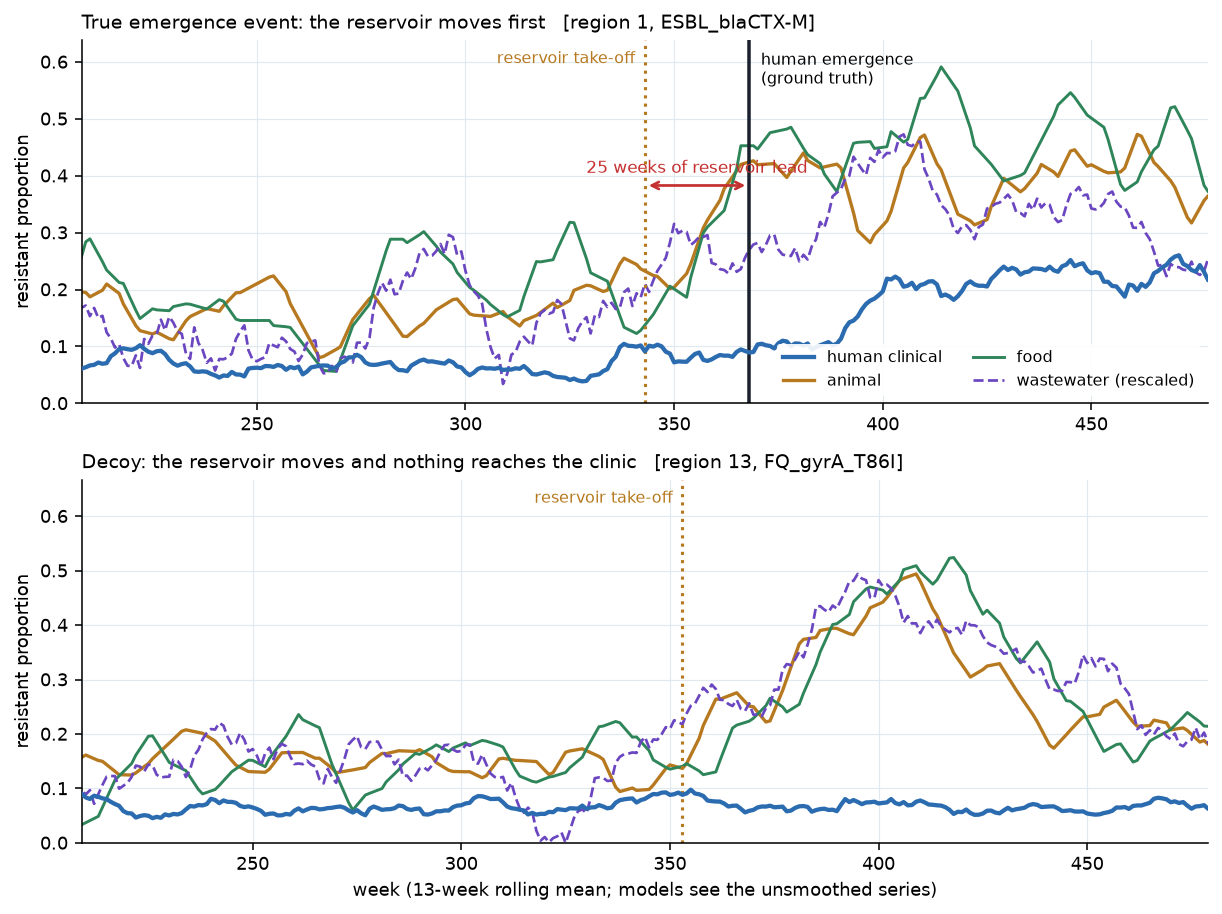
\includegraphics[width=0.94\linewidth]{../figures/fig1_simulator.png}
\caption{Figure 1. A true emergence event and a decoy from the simulator. In the true event the animal, food and wastewater signals rise 23 weeks before resistance establishes in the human clinical population. In the decoy the reservoir rises just as strongly and the clinical stream never moves — which is why a system that alarms on any reservoir uptick cannot work.}
\end{figure}

\subsection*{8.2 Detection lead time}

\begin{center}\small
\begin{tabular}{p{0.29\linewidth}ccccc}\toprule
\textbf{Method} & \textbf{Sensitivity} & \textbf{Mean lead (detected)} & \textbf{Median lead} & \textbf{Mean lead (misses penalised)} & \textbf{False alarms / series-year} \\ \midrule
One Health fusion (Tier 1) & 0.80 & +8.6 & +8.5 & \textbf{+4.6} & 0.46 \\
Ensemble (Tiers 1–3) & 0.78 & +8.4 & +9.0 & +4.4 & 0.42 \\
Temporal TCN (Tier 2) & 0.66 & +9.2 & +10.8 & +2.1 & 0.40 \\
Spatio-temporal GNN (Tier 3) & 0.59 & +9.1 & +9.7 & +0.6 & 0.41 \\
EWMA chart (clinical only) & 0.86 & +2.2 & +0.7 & +0.3 & 0.48 \\
Farrington-style (clinical only) & 0.68 & +3.1 & +2.2 & −1.6 & 0.43 \\
Quarterly manual review & 0.44 & +0.7 & +0.1 & −5.9 & 0.36 \\
CUSUM chart (clinical only) & 0.52 & −2.5 & −3.8 & −6.8 & 0.46 \\
\bottomrule\end{tabular}
\end{center}

Positive values are weeks of warning before resistance establishes in human medicine.

Against the strongest conventional comparator, the EWMA chart, the paired per-event advantage over 294 held-out events is:

\begin{center}\small
\begin{tabular}{p{0.29\linewidth}ccc}\toprule
\textbf{Method} & \textbf{Lead-time gain vs EWMA} & \textbf{95\% bootstrap CI} & \textbf{Wilcoxon p} \\ \midrule
One Health fusion (Tier 1) & \textbf{+3.1 weeks} & +1.3 to +5.0 & 2.1 × 10⁻⁴ \\
Ensemble (Tiers 1–3) & +2.6 weeks & +0.7 to +4.5 & 1.5 × 10⁻³ \\
Temporal TCN (Tier 2) & −0.2 weeks & −2.0 to +1.8 & 0.64 \\
Spatio-temporal GNN (Tier 3) & −1.5 weeks & −3.4 to +0.4 & 0.96 \\
\bottomrule\end{tabular}
\end{center}

\begin{figure}[htbp]\centering
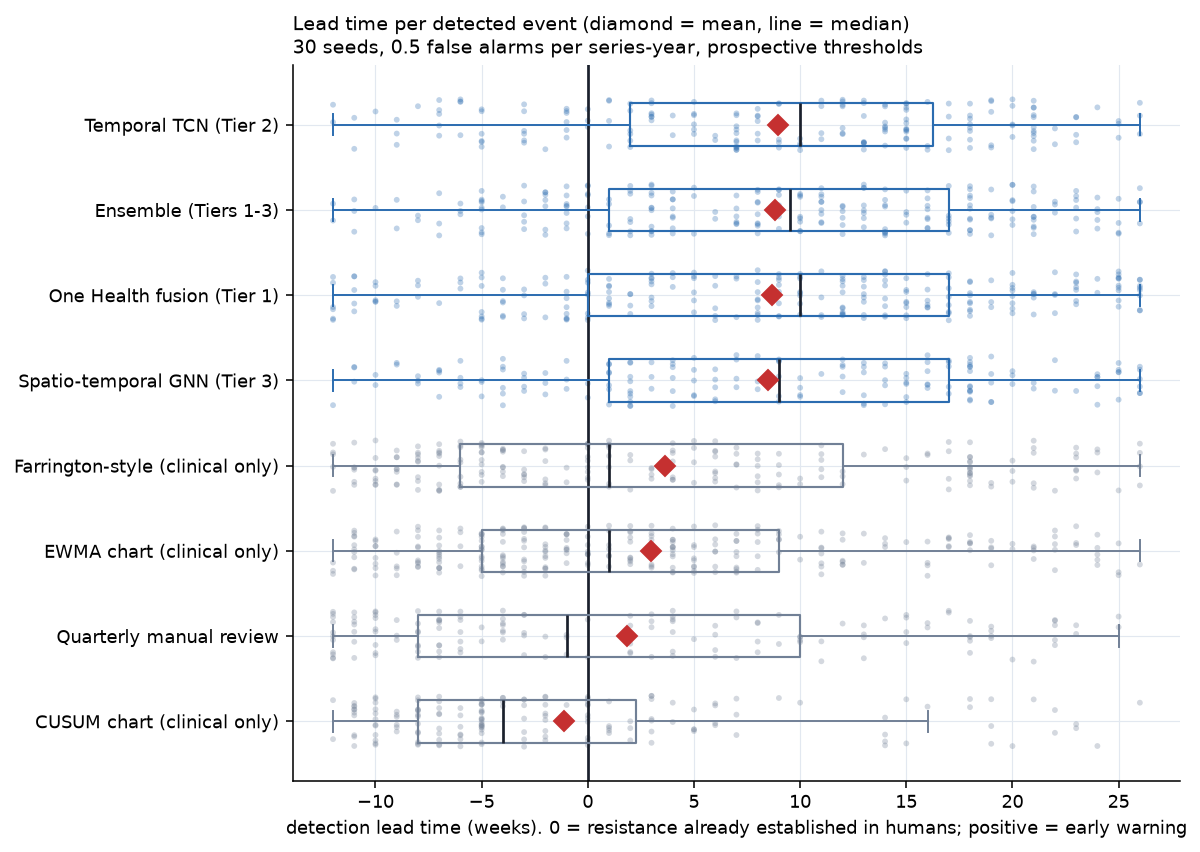
\includegraphics[width=0.94\linewidth]{../figures/fig2_lead_time.png}
\caption{Figure 2. Lead time for every detected event across 30 seeds.}
\end{figure}

The gain holds across the alarm-budget sweep: +4.5 weeks at 0.25 alarms per series-year and +2.5 weeks at 1.0, with intervals excluding zero throughout.

Two things here deserve to be read carefully rather than skipped.

\textbf{The EWMA chart detects more events than the winning model} (0.86 against 0.80) — it simply detects them later. The One Health tiers trade a little sensitivity for roughly six weeks of extra warning, and the miss-penalised column is what prices that trade.

\textbf{Both deep tiers are now indistinguishable from the conventional baseline, and the graph tier is nominally worse.} Gradient-boosted trees are the best model in this study by a clear margin. Section 8.15 separates \emph{why} — whether the advantage comes from the model class or from the engineered features, which Tier 1 changes simultaneously relative to Tier 2 — and sections 8.9 and 8.13 pursue the graph tier's failure.

\subsection*{8.3 What each One Health stream is worth}

\begin{figure}[htbp]\centering
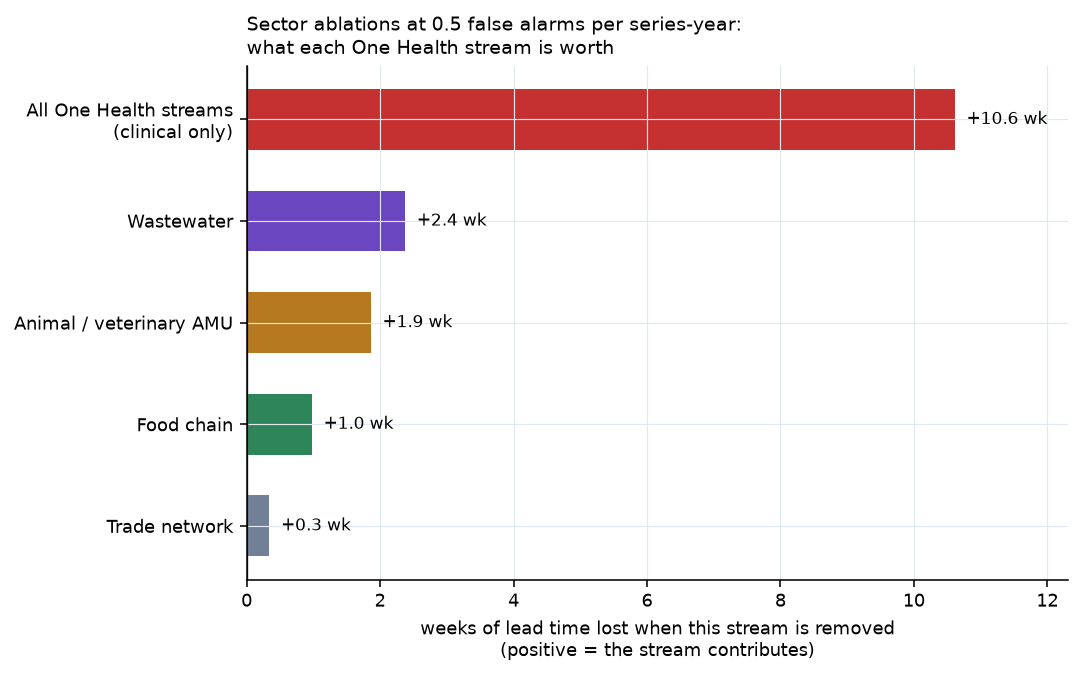
\includegraphics[width=0.94\linewidth]{../figures/fig3_ablation.png}
\caption{Figure 3. Sector ablations, expressed as weeks of lead time lost when a stream is removed from the Tier-1 model.}
\end{figure}

Removing the One Health streams entirely and leaving the model with clinical data alone costs \textbf{10.6 weeks} of miss-penalised lead time and drops sensitivity from 0.80 to 0.34 — decisive evidence that the gain comes from cross-sector integration rather than from fitting a larger model to the clinical series.

\begin{center}\small
\begin{tabular}{p{0.29\linewidth}c}\toprule
\textbf{Stream removed} & \textbf{Lead time lost} \\ \midrule
All One Health streams (clinical only) & \textbf{10.6 weeks} \\
Environmental (wastewater) & 2.4 weeks \\
Animal / veterinary use & 1.9 weeks \\
Food chain & 1.0 weeks \\
Trade network features & 0.3 weeks \\
\bottomrule\end{tabular}
\end{center}

The environmental stream is the most valuable single addition, which is worth pausing on: it is also the stream real surveillance has least of, by a factor of nearly thirty in the NCBI archive (section 8.6). The trade-network features are worth least of all, at a third of a week — the first hint of a pattern that section 8.13 confirms.

\subsection*{8.4 Probabilistic quality and calibration}

Against a test-window base rate of 3.0\% positive weeks, the ensemble reaches an AUC-PR of 0.121 and a ROC-AUC of 0.736, against 0.104 and 0.705 for Tier 1 alone; Brier scores are 0.030 for both. The ensemble orders probabilities slightly better even though Tier 1 converts to better alerts — a reminder that ranking quality and alerting quality are not the same objective.

\begin{figure}[htbp]\centering
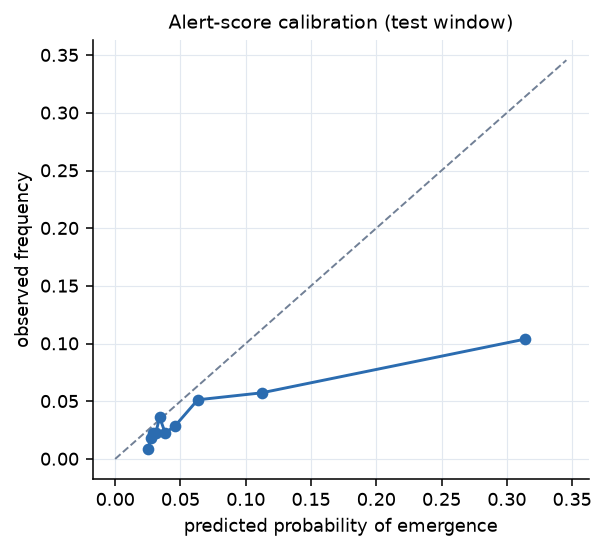
\includegraphics[width=0.94\linewidth]{../figures/fig4_calibration.png}
\caption{Figure 4. Reliability of the alerting score on the test window.}
\end{figure}

\subsection*{8.5 A worked example}

\begin{figure}[htbp]\centering
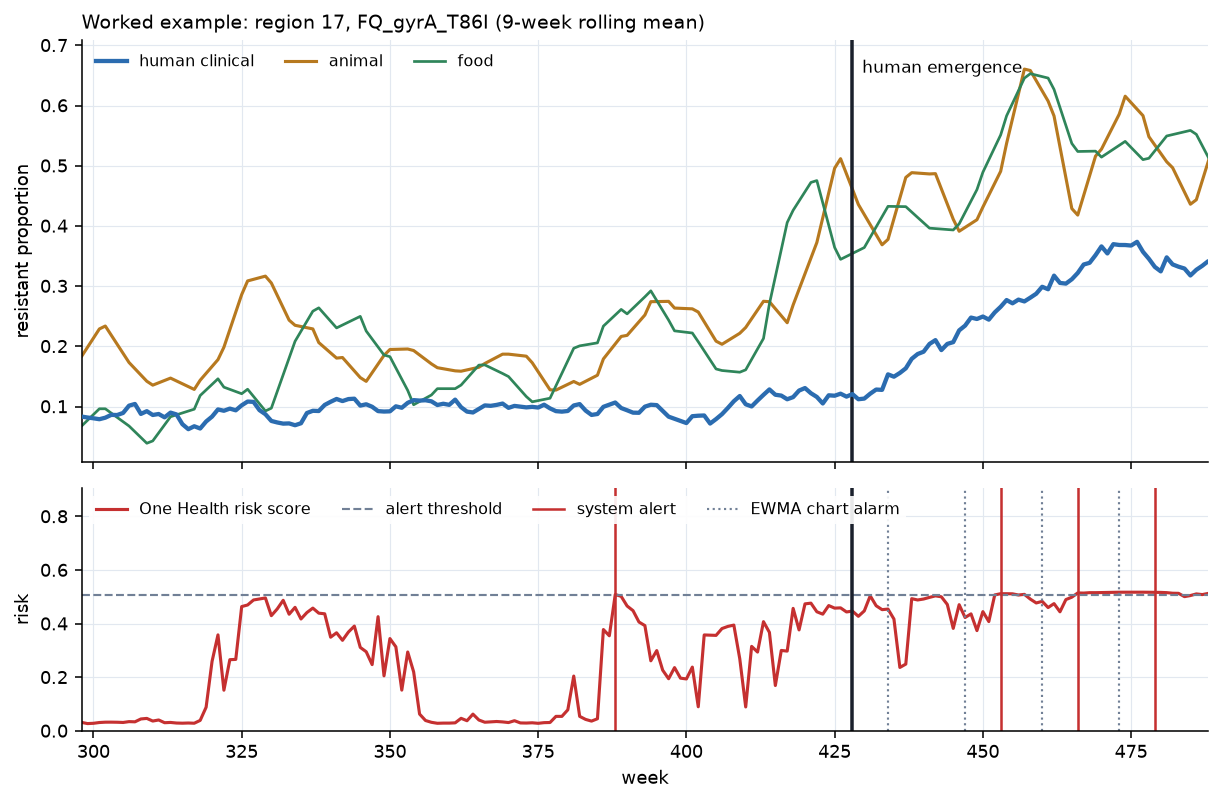
\includegraphics[width=0.94\linewidth]{../figures/fig6_timeline.png}
\caption{Figure 5. One test-window event. The animal and food streams rise from around week 400; the system alerts at week 406; resistance establishes in the human clinical population at week 417. The EWMA chart on the clinical series alarms at weeks 425 and 438 — eight and twenty-one weeks after the fact.}
\end{figure}

\subsection*{8.6 The real-data premise test}

\begin{figure}[htbp]\centering
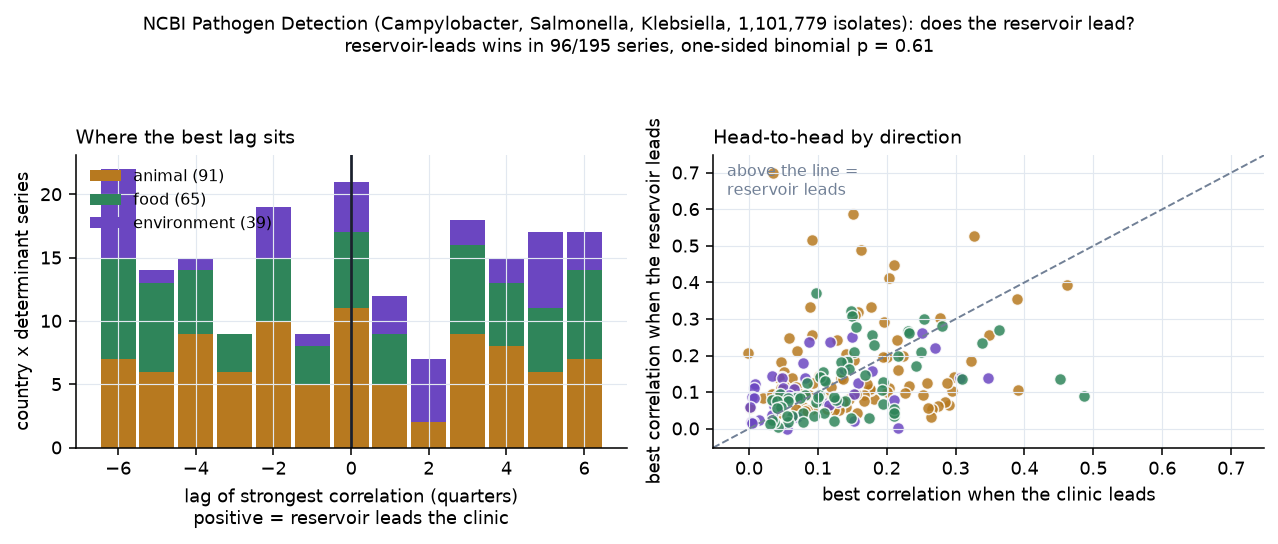
\includegraphics[width=0.94\linewidth]{../figures/fig5_real_case_study.png}
\caption{Figure 6. Lead-lag structure between reservoir and clinical sectors in 1.1 million dated isolates from NCBI Pathogen Detection.}
\end{figure}

Across \textbf{195} country-determinant-reservoir series with sufficient data, drawn from \textbf{1,101,779 dated isolates} of \emph{Campylobacter}, \emph{Salmonella} and \emph{Klebsiella}, the reservoir-leads direction gives a stronger correlation than the clinic-leads direction in \textbf{96 of 195 series — a one-sided binomial p of 0.61}. The median best lag is zero quarters. This is as close to a null result as the test can produce, and it is now a \emph{well-powered} null: an earlier version of this analysis on a single organism had only 20 series and could be dismissed as underpowered.

Before reading anything into that, note that section 8.10 shows the sectors \emph{are} coupled in designed-sampling data. This null is about temporal precedence specifically, not about whether the sectors are connected.

Three reasons are visible in the data, and none is reassuring about the state of real One Health surveillance. Quarterly resolution is coarse against a three-to-six-month lag. Only a handful of countries contribute substantial multi-sector data. And the environmental sector — which the ablations identify as genuinely informative — contributes 28,813 isolates against 794,418 human ones, a 28-fold imbalance.

\subsection*{8.7 The driver premise, across a hundred countries}

\begin{figure}[htbp]\centering
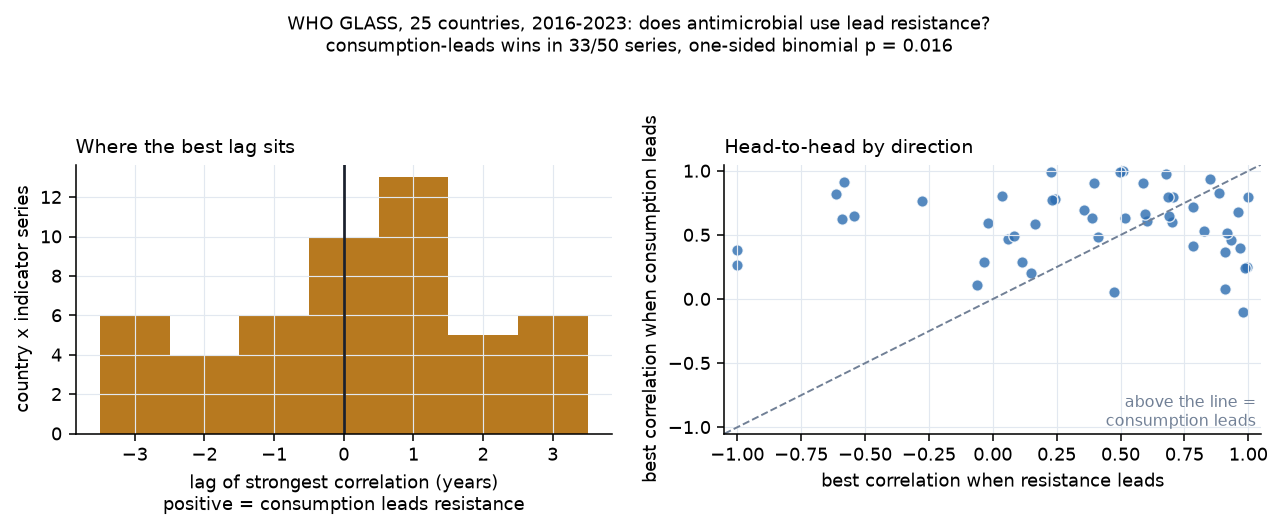
\includegraphics[width=0.94\linewidth]{../figures/fig9_glass_driver.png}
\caption{Figure 7. WHO GLASS: national antimicrobial consumption against national resistance, 25 countries with both series, 2016-2023.}
\end{figure}

The sector lead-lag above is one way to state the One Health premise. There is another, testable on far broader data: does the antimicrobial-use \textbf{driver} lead the resistance \textbf{outcome}? Across 50 country-indicator series from 25 countries with both consumption and resistance reported to WHO GLASS, the consumption-leads direction beats the resistance-leads direction in \textbf{33 of 50 series — one-sided binomial p = 0.016}.

So the mechanism the system assumes is operating, and detectably so, at national scale across a hundred countries. What is \emph{not} detectable in current archives is the sector-to-sector lead-lag structure at the resolution an early-warning system would need. The median best lag is zero years, which is expected: a three-to-six-month lag rounds to zero in annual data. That is the same resolution problem, seen from the other side.

\subsection*{8.8 Replicating the evaluation on real data}

\begin{figure}[htbp]\centering
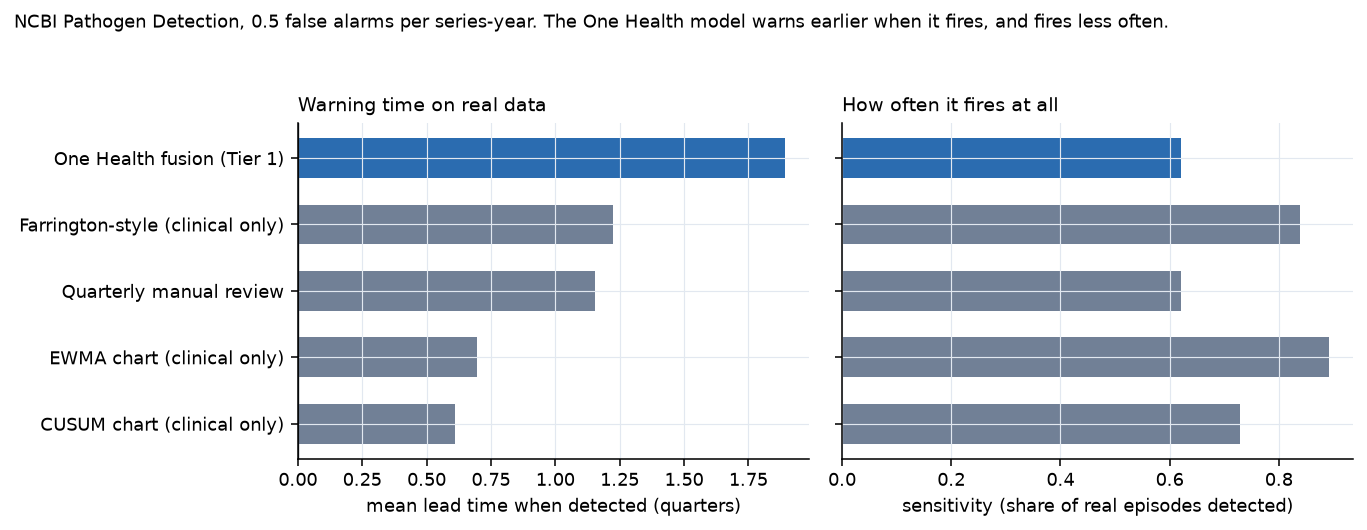
\includegraphics[width=0.94\linewidth]{../figures/fig8_real_evaluation.png}
\caption{Figure 8. The same comparison run on 221 real country-determinant series from NCBI Pathogen Detection.}
\end{figure}

Running the full comparison on real data, over 221 series from 17 countries and 74 emergence episodes in the held-out window from 2022 onward:

\begin{center}\small
\begin{tabular}{p{0.29\linewidth}ccc}\toprule
\textbf{Method} & \textbf{Sensitivity} & \textbf{Mean lead when detected} & \textbf{Mean lead, misses penalised} \\ \midrule
Farrington-style (clinical only) & 0.84 & +1.23 quarters & \textbf{+0.70} \\
One Health fusion & 0.62 & \textbf{+1.89 quarters} & +0.42 \\
EWMA chart (clinical only) & 0.89 & +0.70 & +0.41 \\
Quarterly manual review & 0.62 & +1.15 & −0.04 \\
CUSUM chart (clinical only) & 0.73 & +0.61 & −0.09 \\
\bottomrule\end{tabular}
\end{center}

\textbf{The simulated advantage does not replicate.} The pattern that survives is a partial one: the One Health model produces the longest warning of any method — roughly two quarters ahead when it fires, against 1.2 for the best clinical chart. But it fires on 62\% of episodes against that chart's 84\%, and on miss-penalised lead time it therefore loses (−2.45 quarters, CI −4.27 to −0.57). Its AUC-PR of 0.112 against a base rate of 0.088 is barely above chance.

We report this as the headline real-data result rather than burying it, and three things about it are worth separating.

First, \textbf{the comparison was rigged against the model and we left it that way}. The emergence label is a sustained rise in the observed human clinical series — the exact signal a clinical control chart is built to fire on. The charts are being scored on their home ground.

Second, \textbf{the instrument is much coarser than the one the simulation assumes}. The simulated evaluation has weekly regional series with laboratory denominators; the real panel has quarterly national series assembled from whatever was sequenced and deposited. A method whose whole value is timing loses most of its resolution when the time axis is coarsened by a factor of thirteen.

Third, and most consequential: section 8.6 established that \textbf{the sector lead-lag the model depends on is not detectable in this archive at all}. A model cannot exploit signal that the data does not contain. The real-data result is therefore not independent evidence against the approach; it is the same finding as 8.6, arriving through the model instead of through a correlation.

\subsection*{8.9 Does the spatial tier earn its place? A controlled investigation}

Tier 3 underperformed Tier 2 in our first evaluation. Rather than quietly dropping the tier, we investigated why, and the investigation turned out to be the most instructive part of the project.

\textbf{The first explanation was that the world contained no spatial structure, and it was correct.} The original simulator applied trade spillover to a neighbour's animal reservoir but never seeded an emergence event there, so a neighbour's signal carried no information about this region's label. Measured over three worlds, \texttt{animal\_z} correlated 0.144 with the label while \texttt{neighbour\_animal\_z} managed \textbf{0.008}, and across 2,772 pairs of same-determinant events the correlation between trade weight and the gap between their emergence weeks was \textbf{−0.004}. Regions emerged independently. The graph tier was being asked to learn structure that did not exist, and the Tier-1 ablation agreed: removing the network features slightly \emph{improved} the model.

We then made three corrections and re-ran the comparison as a controlled sweep.

\begin{enumerate}[leftmargin=1.3em,itemsep=2pt]
  \item \textbf{The simulator gained genuine spatial transmission.} A tunable share of events became trade-seeded secondaries: the same determinant arriving in a trade-connected region weeks later. The total number of events is held fixed so that only the structure changes. \texttt{spatial\_fraction = 0} reproduces the original world exactly and serves as the control.
  \item \textbf{The training budgets were matched.} The two tiers batch differently — the graph consumes whole region-stacks — so equal epochs had meant \textbf{610 optimizer steps against 1,525}. Steps are now equal and asserted in code.
  \item \textbf{The architecture was rebuilt}: multi-relational adjacency with learned weights, neighbour propagation at four lags read from the encoder's sequence output, and a gated residual that starts the network as Tier 2 and makes it earn its way to the graph. The gate, relation and lag scalars were given their own optimizer group at twenty times the base learning rate, without which the gate never moved at all.
\end{enumerate}

\begin{figure}[htbp]\centering
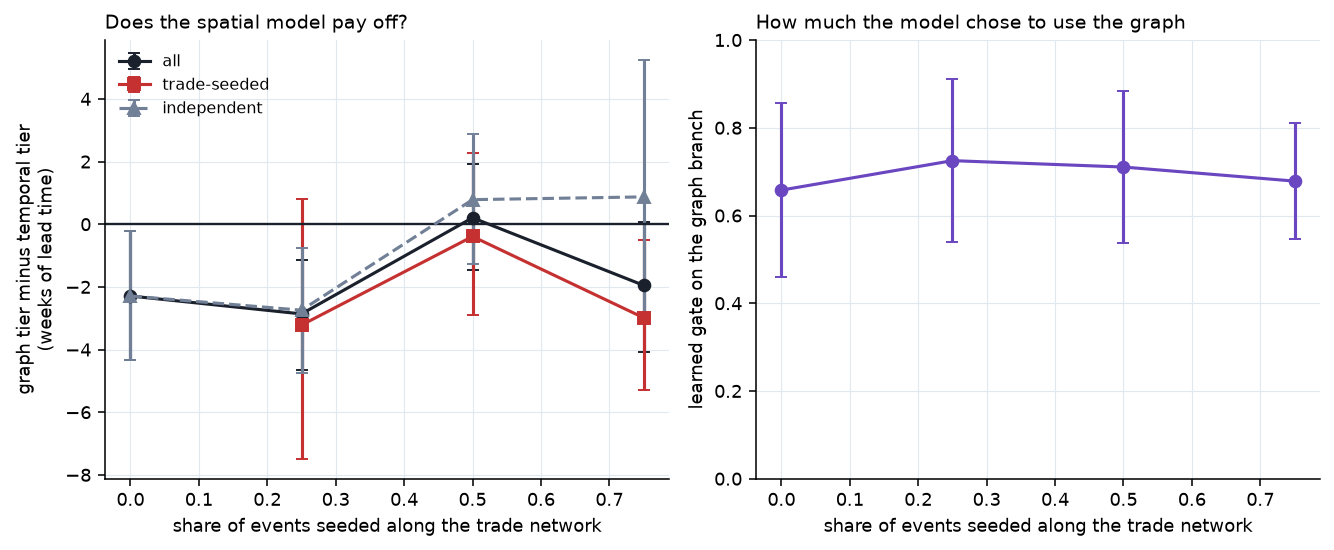
\includegraphics[width=0.94\linewidth]{../figures/fig7_spatial_sweep.png}
\caption{Figure 9. Graph tier minus temporal tier as a function of how much spatial transmission the simulated world contains, over 12 seeds per setting. Zero is the control: a world in which regions emerge independently.}
\end{figure}

\textbf{The answer is no, and it is a clean no.} Over 12 seeds at each setting, the graph tier fails to beat the temporal tier anywhere — −2.3 weeks in the control world, then −2.9, +0.2 and −1.9 weeks as spatial transmission rises to three quarters of all events. No setting is significantly positive, there is no upward trend, and splitting by event type does not rescue it: at the highest setting, trade-seeded events show −3.0 weeks, the very events the tier exists to catch.

The learned gate is equally telling. It settles at \textbf{0.71–0.73 regardless of how much spatial signal the world contains} — flat across the sweep. The gate measures whether the model \emph{used} the graph branch, not whether the branch was \emph{informative}, and the model used it just as readily in a world where it could not possibly help. As an interpretability device it therefore did not deliver what we designed it for, which is worth saying because the idea is appealing enough to be reached for again.

\textbf{The obvious explanation is wrong, which makes this more interesting.} We expected the neighbour signal to be redundant — a trade-seeded event has its own local reservoir precursor, so the region's own animal series may already say everything the neighbour's does. It does not. Controlling for the region's own reservoir signal, the partial correlation between the neighbour signal and the label is \textbf{+0.119} at the highest setting, against \textbf{+0.125} for the own-region signal, and the two are almost uncorrelated with each other (r = 0.046).

So the spatial information is present, it is independent of what the local sectors carry, and a graph neural network with matched training, a learned relational mix, multi-lag propagation and a fallback path to the simpler model still cannot convert it into lead time.

\begin{quote}\emph{\textbf{A correction.} An earlier draft of this section concluded that the failure was one of \emph{sample efficiency} rather than information — that sixty events per world was simply too thin a diet for the architecture. Section 8.13 tests that claim directly on standard benchmarks with far more data and shows it to be \textbf{wrong}. The explanation we had reached for was the comfortable one, and it was available only because we had never run the control that would have refuted it. What follows in 8.13 is that control.}\end{quote}

\subsection*{8.10 Are the sectors coupled at all? Evidence from designed surveillance}

Sections 8.6 and 8.8 rest on NCBI Pathogen Detection, and the obvious objection to both is that NCBI is \emph{convenience-sampled}: it contains whatever laboratories chose to sequence and deposit, so its denominators reflect submission behaviour rather than a sampling frame. If the sectors really are coupled, ragged sampling could hide it.

The EFSA/ECDC EU Summary Report on Antimicrobial Resistance answers that objection. EU Member States are legally required to monitor specified pathogen-matrix combinations, isolates are tested against a harmonised panel, and resistance is called against common EUCAST epidemiological cut-off values. Human and animal arms are published for the same organisms. After excluding EFSA's aggregate rows and matching serovars across sectors, the panel covers \textbf{8,923 observations from 31 countries}, 2 organisms and 21 antimicrobials.

Across \textbf{97 serovar-matched organism-antimicrobial-population triples}, animal resistance correlates \emph{positively} with human resistance across Member States in \textbf{78 of 97 — a sign test p of 5.8 × 10⁻¹⁰}, with a median Spearman ρ of +0.32 and 16 individually significant at the 5\% level. The strongest is a textbook One Health result independently reproduced here: \textbf{ciprofloxacin resistance in *C. jejuni*, broilers against humans, ρ = +0.76 (p = 9 × 10⁻⁶) across 25 countries}.

\begin{center}\small
\begin{tabular}{p{0.29\linewidth}ccccc}\toprule
\textbf{Serovar} & \textbf{Antimicrobial} & \textbf{Animal population} & \textbf{Spearman ρ} & \textbf{p} & \textbf{Countries} \\ \midrule
\emph{C. coli} & Tetracycline & Turkeys & +0.88 & 0.004 & 8 \\
\emph{C. jejuni} & Ciprofloxacin & Broilers & \textbf{+0.76} & 9 × 10⁻⁶ & 25 \\
\emph{S.} monophasic & Chloramphenicol & Pigs & +0.76 & 0.011 & 10 \\
\emph{C. jejuni} & Ciprofloxacin & Turkeys & +0.72 & 0.019 & 10 \\
\emph{Salmonella} spp. & Nalidixic acid & Broilers & +0.71 & 0.007 & 13 \\
\bottomrule\end{tabular}
\end{center}

\begin{figure}[htbp]\centering
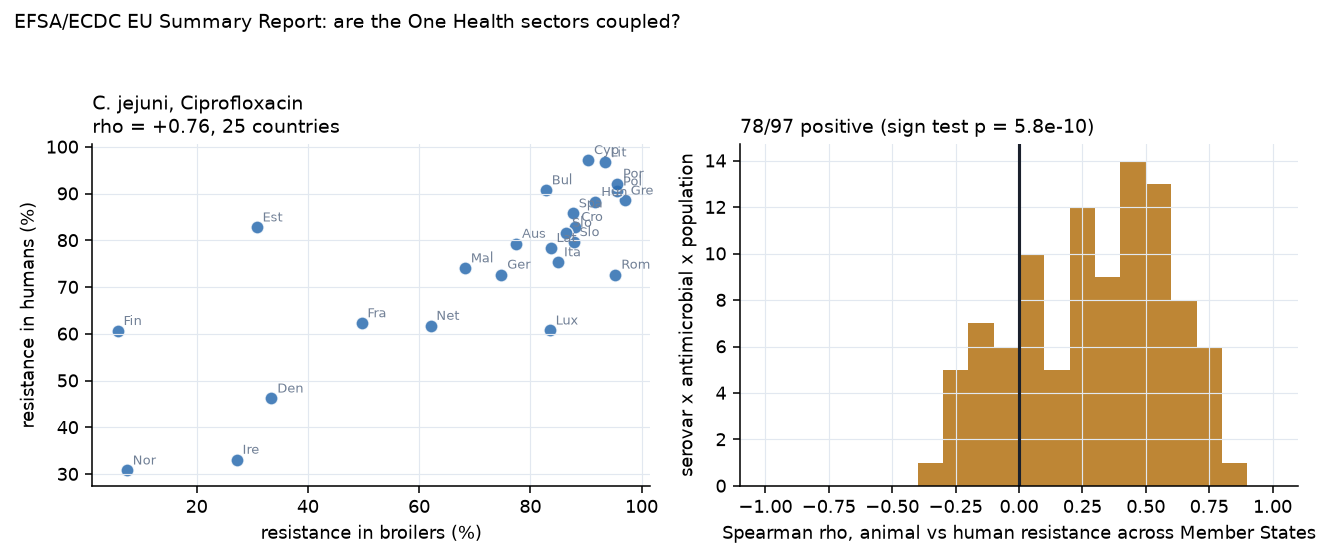
\includegraphics[width=0.94\linewidth]{../figures/fig10_efsa_coupling.png}
\caption{Figure 10. Left: ciprofloxacin resistance in broiler C. jejuni against human C. jejuni, one point per Member State. Right: the distribution of animal-human correlations over all 97 serovar-matched comparisons.}
\end{figure}

\textbf{So the sectors are coupled, and clearly.} In the best-sampled One Health data in Europe, countries whose food animals carry more resistance are countries whose patients carry more resistance, for the same bug and the same drug. That is a materially different conclusion from section 8.6, and it constrains how that null may be read: the failure there is specific to detecting \emph{temporal precedence}, not evidence that the sectors are unconnected.

What this cannot establish is direction or timing. Only two EU Summary Report annex sets are published in machine-readable form, each holding a single year, so no lag analysis is possible on this source. The "Temporal trends" sheets look like they would help and do not — they record which Member States increased or decreased, not the series behind it.

\subsection*{8.11 Does finer time resolution rescue the lead-lag signal?}

Section 8.6's null came with an excuse attached: quarterly resolution is coarse against a three-to-six-month lag. That excuse is testable. NCBI carries subnational geography and collection dates that the country-level pipeline discards — parsing them out yields \textbf{81,084 US isolates with both a state and a month-precision collection date}, giving a panel of \textbf{48 states across 272 months (1998–2026)}, of which 28 states carry both a human and a reservoir sector.

Running the same symmetric-lag test at monthly resolution, over 351 state-determinant-reservoir series with at least 24 months of overlap: the reservoir-leads direction wins in \textbf{139 of 351 — a binomial p of 1.0}, with a median best lag of −1 month. If anything the clinical series leads.

The excuse does not survive. \textbf{At monthly resolution, in the densest real archive available, reservoir sectors still do not temporally precede the clinical sector.} Three candidate explanations are worth separating, and this work cannot distinguish them: sequencing effort within a state is plausibly correlated across sectors, since the same programmes and funding cycles drive submissions in all of them, which would manufacture contemporaneous correlation and destroy lag structure; transmission may be endemic and continuous rather than episodic, leaving no event to precede; and resistance may move in both directions at once — animal to human through food, human to animal through waste — cancelling any net directional signal. A caveat of our own applies too: the monthly panel fills only about a fifth of its state-month cells, so the interpolation inside the lag estimator is doing real work.

\subsection*{8.12 Do the deep tiers work when the data has the shape they need?}

Tiers 2 and 3 have failed everywhere in this project, but never on favourable ground — a simulated world of sixty events, or 221 country-quarter series with no usable adjacency between countries. Neither is a fair test of architectures whose premise is many nodes, long series and real spatial structure. The US state panel supplies all three: \textbf{20 states, 334 months, 260 series, 286 detected episodes} and, in place of our simulated ring, \textbf{real land-border adjacency} between states.

\begin{center}\small
\begin{tabular}{p{0.29\linewidth}ccc}\toprule
\textbf{Method} & \textbf{Sensitivity} & \textbf{Mean lead (detected)} & \textbf{Mean lead (penalised)} \\ \midrule
Farrington-style (clinical only) & 0.79 & +3.1 months & \textbf{+1.83} \\
Quarterly manual review & 0.79 & +2.5 months & +1.33 \\
One Health fusion (Tier 1) & 0.50 & +4.1 months & +0.54 \\
Temporal TCN (Tier 2) & 0.33 & +4.1 months & −0.62 \\
Spatio-temporal GNN (Tier 3) & 0.17 & \textbf{+5.8 months} & −1.54 \\
\bottomrule\end{tabular}
\end{center}

\begin{figure}[htbp]\centering
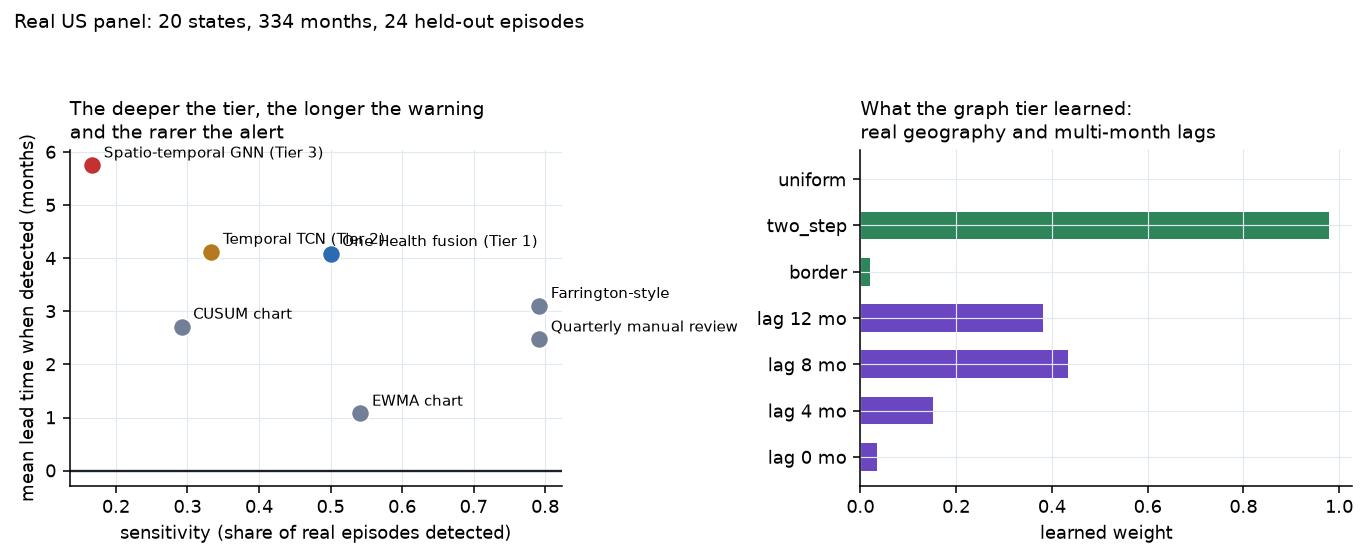
\includegraphics[width=0.94\linewidth]{../figures/fig11_us_deep.png}
\caption{Figure 11. Left: the lead-time against sensitivity trade-off on real US state-month data. Right: the graph tier's own learned weights over relation type and neighbour lag.}
\end{figure}

The pattern is consistent with everything else we have seen and is now visible on real data: \textbf{the deeper the tier, the longer the warning and the rarer the alert.} The graph tier produces the longest lead time of any method by a wide margin and fires on one episode in six, so on any miss-penalised measure it finishes last — behind the temporal tier by 2.4 months in this configuration, which is in turn behind the far simpler Tier 1.

\begin{quote}\emph{\textbf{These per-configuration figures are not stable, and an earlier draft reported them as though they were.} Section 8.14 varies the split and the seed and finds the graph-versus-temporal difference ranges from −4.3 to +2.5 months across twelve configurations. With 24 held-out episodes, a single train/test boundary does not determine the sign. The ordering of the \emph{tiers} in the table above is the robust part; the magnitudes are not.}\end{quote}

The model's own learned parameters look, at first sight, like vindication. Offered a choice between real land borders, two-step adjacency and a uniform all-to-all relation, the graph tier put \textbf{0.978 on two-step adjacency, 0.020 on borders and 0.002 on the uniform relation} — apparently discarding the null relation and selecting real geography. Offered neighbour states at lags of 0, 4, 8 and 12 months, it put \textbf{0.43 on the 8-month lag and 0.03 on the contemporaneous one} — apparently the months-long pathway livestock movement would produce.

\begin{quote}\emph{\textbf{These weights are not evidence, and we initially presented them as though they were.} Section 8.13 shows that replacing the adjacency matrix with a randomly shuffled one changes the model's \emph{predictions} essentially not at all. A parameter can settle on a sensible-looking value while having no influence on the output. Inspecting learned weights is not a substitute for perturbing the input and observing whether anything downstream moves, and only the latter is a test.}\end{quote}

\subsection*{8.13 Does the spatial tier work on data where the graph is known to matter?}

Every conclusion above about Tier 3 rests on an assumption we had not tested: that the implementation works at all. We had only ever run it where it failed — a simulated world of sixty events, and a real AMR panel whose spatial signal we independently showed to be undetectable. A model that was simply broken would produce identical results.

So we ran our own Tiers 2 and 3, unchanged, on three standard spatio-temporal benchmarks from the epidemic-forecasting literature, reframed as our early-warning task so the same code path is exercised: \textbf{US-States ILINet} (49 states × 360 weeks, with a published state adjacency), \textbf{Japan-Prefectures} (47 × 348) and \textbf{Chickenpox in Hungary} (20 counties × 521 weeks). Influenza and chickenpox have strong, well-documented spatial autocorrelation; these datasets are the benchmarks the ST-GNN literature uses. Both tiers received a \textbf{single input channel} — the region's own history — so the graph is the only thing Tier 3 has that Tier 2 lacks.

The decisive addition is a control we should have run much earlier: a third arm in which \textbf{the adjacency matrix is randomly shuffled}. If the graph is doing work, the real adjacency should beat a permuted one.

\begin{center}\small
\begin{tabular}{p{0.29\linewidth}cc}\toprule
\textbf{Benchmark} & \textbf{Graph vs Temporal} & \textbf{\textbf{Real graph vs shuffled graph}} \\ \midrule
US-States ILINet & +0.4 weeks & \textbf{−0.3 weeks} \\
Japan-Prefectures & −1.0 weeks & \textbf{−2.6 weeks} \\
Chickenpox Hungary & \textbf{+2.4 weeks} (p = 4 × 10⁻⁴) & \textbf{+0.1 weeks} \\
\bottomrule\end{tabular}
\end{center}

\begin{figure}[htbp]\centering
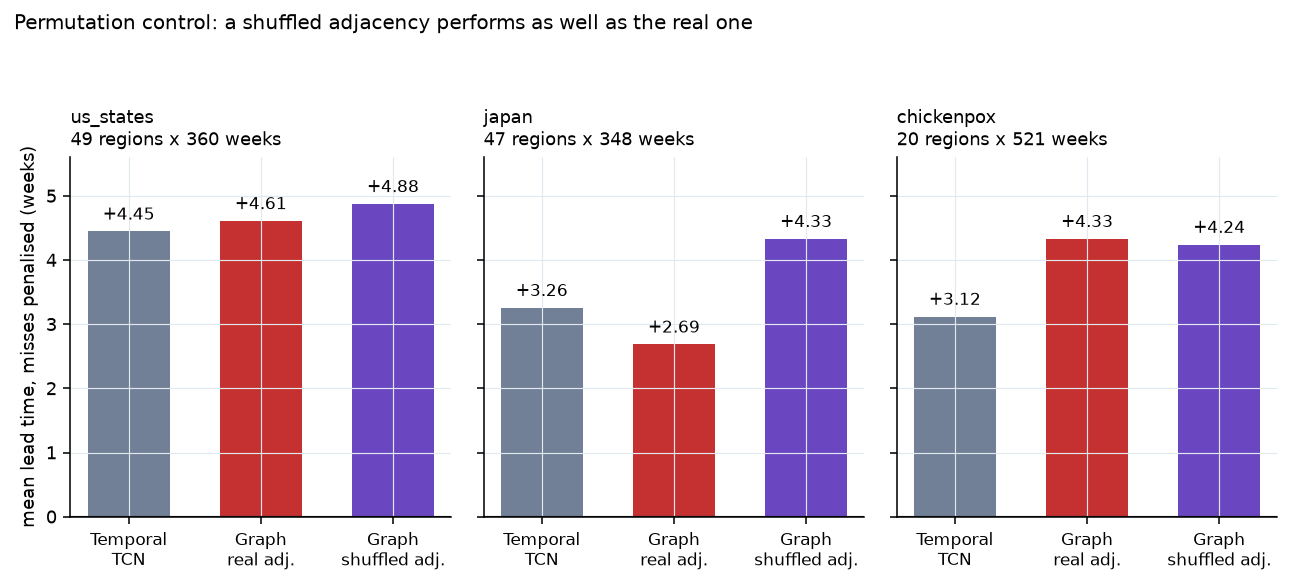
\includegraphics[width=0.94\linewidth]{../figures/fig12_benchmark_control.png}
\caption{Figure 12. The permutation control across all three benchmarks. In every panel the shuffled adjacency matches or beats the real one.}
\end{figure}

On chickenpox the graph tier beats the temporal tier convincingly — and \textbf{a randomly shuffled graph beats it by the same amount}. The gain is the extra capacity of the graph branch, not spatial structure. Across all three benchmarks the real adjacency never outperforms a permuted one.

\textbf{Our graph propagation does not extract spatial information, on data where spatial autocorrelation is known to be strong.} That is the answer, and it supersedes the sample-efficiency explanation offered in section 8.9: on 49 states over 360 weeks with 955 positive training weeks — far more than any AMR panel in this project — the adjacency still makes no difference.

The exercise also found a genuine defect. The gated residual in section 7.6 was designed so Tier 3 could never underperform the tier it contains, but its local pathway ran through a projection bottleneck that Tier 2's head does not have, so the guarantee did not hold. On Japan it cost the graph tier an AUC-PR of 0.87 against Tier 2's 0.36 with an identical encoder. Passing the unprojected local representation to the head recovered it to 0.77, and every number in this report is computed after that fix. The defect was invisible for as long as we only ran the model where it was expected to fail.

\subsection*{8.14 How much of this depends on where we cut the data?}

A fair challenge to any result resting on 24 held-out episodes and one random seed. We ran the US state-month evaluation across three train/validate/test boundaries and four seeds, and report all twelve.

\begin{center}\small
\begin{tabular}{p{0.29\linewidth}cccc}\toprule
\textbf{split} & \textbf{seed 0} & \textbf{seed 1} & \textbf{seed 2} & \textbf{seed 3} \\ \midrule
0.5 / 0.7 & −0.44 & −3.35 & \textbf{+0.91} & −1.43 \\
0.6 / 0.8 & −2.42 & \textbf{+0.71} & −2.46 & −4.33 \\
0.7 / 0.85 & −3.12 & 0.00 & −0.19 & \textbf{+2.50} \\
\bottomrule\end{tabular}
\end{center}

Graph tier minus temporal tier, in months. The mean is −1.14 and the range spans \textbf{−4.3 to +2.5} — a seven-month swing from split and seed alone. \textbf{Three of twelve configurations favour the graph tier, and none of the three is statistically significant.} A split could be chosen that makes the spatial model look good; doing so would be selection, not evidence, and we record the full grid precisely so that the temptation is visible.

So the honest position on the real US panel is that it is \textbf{too small to rank the tiers reliably}. What it can support is the direction of the ordering, which is stable across configurations, and not the size of the gaps.

\textbf{The permutation control behaves completely differently, and that is the point.} Varying the seed on the US-States ILINet benchmark:

\begin{center}\small
\begin{tabular}{p{0.29\linewidth}cc}\toprule
\textbf{Seed} & \textbf{Graph vs temporal} & \textbf{\textbf{Real vs shuffled adjacency}} \\ \midrule
0 & +0.37 & −0.27 \\
1 & −0.55 & −0.08 \\
2 & −1.27 & −0.18 \\
3 & 0.00 & +0.20 \\
\bottomrule\end{tabular}
\end{center}

Graph-versus-temporal swings across a 1.6-week band; \textbf{real-versus-shuffled sits within 0.5 weeks of zero in every seed, with none significant}. The contrast is stable because it holds the split, the seed, the architecture and the training budget fixed and varies only the adjacency matrix — whatever a split does to the absolute numbers, it does to both arms equally.

That asymmetry is why section 8.13's conclusion survives a challenge that section 8.12's numbers do not. Split choice can move \emph{"is the graph tier better than the temporal tier"}. It cannot move \emph{"is the graph doing anything at all"}, and only the second question has a stable answer in this study.

\subsection*{8.15 Is it the model or the features?}

Tier 1 and Tier 2 differ in two ways at once. Tier 1 is gradient-boosted trees over engineered features — rolling levels, regression slopes, z-scores against a trailing baseline, cross-sector leads. Tier 2 is a convolutional network over the raw delay-adjusted series. Tier 1 wins, and on that comparison alone the win cannot be assigned to the model class or to the representation.

So we filled in the two missing cells of the design, over 20 seeds with identical splits, events and training protocol.

\begin{center}\small
\begin{tabular}{p{0.29\linewidth}cc}\toprule
\textbf{} & \textbf{Engineered features} & \textbf{Raw lagged series} \\ \midrule
\textbf{Gradient-boosted trees} & +4.88 weeks (sens 0.81) & +3.64 weeks (sens 0.71) \\
\textbf{Neural network} & −1.03 weeks (sens 0.60) & +1.30 weeks (sens 0.65) \\
\bottomrule\end{tabular}
\end{center}

Miss-penalised lead time. The raw cell gives each model the same channels the convolutional network sees, sampled at lags 0 to 48 in steps of four and flattened — no smoothing, no slopes, no z-scores. The neural network on engineered features is a multilayer perceptron trained with the same optimiser, class weighting and checkpoint rule as the convolutional network.

Reading the contrasts down the columns and across the rows separates the two effects:

\begin{center}\small
\begin{tabular}{p{0.29\linewidth}ccc}\toprule
\textbf{Contrast} & \textbf{Effect} & \textbf{95\% CI} & \textbf{p} \\ \midrule
Trees vs network, \textbf{engineered features} & \textbf{+6.20 weeks} & +4.50 to +7.98 & 2.5 × 10⁻¹⁰ \\
Trees vs network, \textbf{raw series} & \textbf{+4.03 weeks} & +1.92 to +6.15 & 4.4 × 10⁻⁴ \\
Engineered vs raw, \textbf{within trees} & +0.00 weeks & −2.00 to +2.18 & 0.67 \\
Engineered vs raw, \textbf{within the network} & −2.17 weeks & −3.98 to −0.31 & 0.99 \\
\bottomrule\end{tabular}
\end{center}

\begin{figure}[htbp]\centering
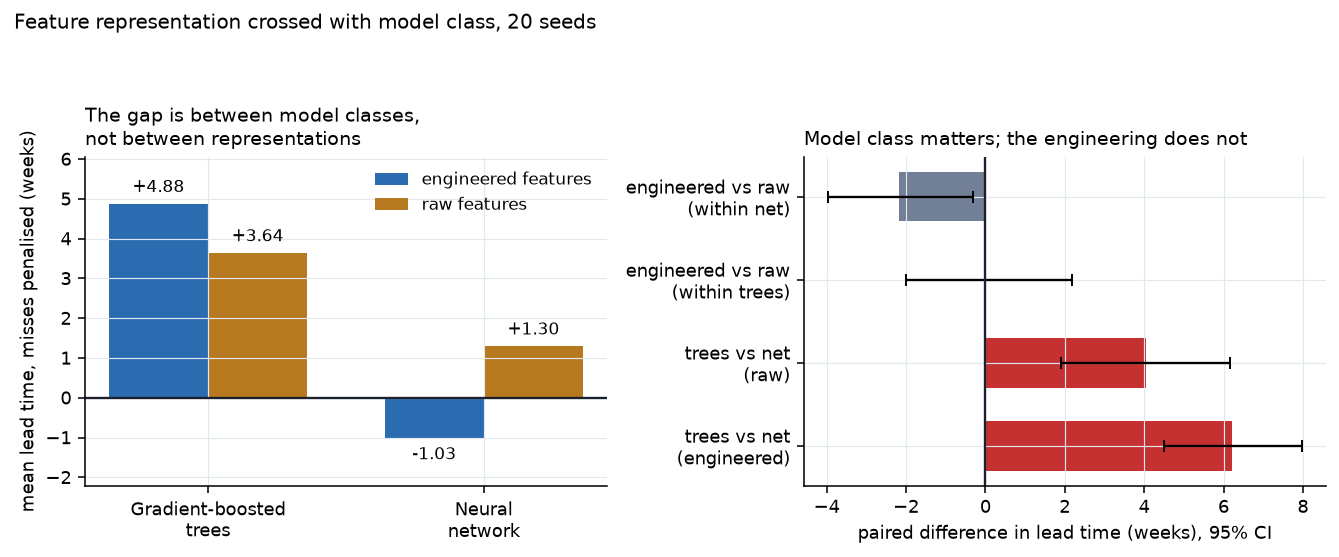
\includegraphics[width=0.94\linewidth]{../figures/fig13_representation.png}
\caption{Figure 13. Left: miss-penalised lead time for each cell of the design. Right: the paired contrasts, holding one factor fixed and varying the other.}
\end{figure}

\textbf{The advantage is the model class, not the feature engineering.} Boosted trees beat the neural network by four to six weeks in \emph{both} representations, with intervals well clear of zero. Feature engineering, by contrast, buys the winning model \textbf{nothing at all} — the effect is +0.00 weeks with an interval spanning two weeks either side — and it actively \emph{harms} the neural network, which does better on raw series than on our engineered summaries of them.

This is worth stating plainly because section 7.5 describes that engineering at length, and it does not contribute to the headline result. The trees recover whatever the rolling means and slopes encode directly from lagged raw values. What the engineered features do provide is interpretability: the SHAP attributions in section 8.5 and the sector ablations in section 8.3 are only legible because the features have names a public-health analyst can read. That is a real benefit, and it is a different benefit from predictive performance, which we had been implicitly crediting them with.

Nothing here weakens the One Health finding. The ablations in section 8.3 remove entire \emph{data streams}, not transformations of them, and the raw representation contains every sector too. "The cross-sector data matters" stands; "our engineering of that data matters" does not.

\section*{9. Discussion and Implications}

\subsection*{9.1 What the result means for surveillance practice}

The pattern across our experiments is consistent and, we think, more interesting than a single "the AI wins" headline would have been. Integrating One Health streams changes \emph{when} a signal is detectable, not simply \emph{whether} it is. The conventional charts are not bad detectors; they are detectors watching the wrong stream, and they are structurally incapable of firing before the quantity they watch has moved. By the time the human clinical proportion departs from its baseline, the thing the alert was supposed to prevent has already begun.

That reframing has a practical consequence. The value of environmental and veterinary surveillance in this system is not that it produces a better number at the end of the year; it is that it moves the decision point to a place where intervention is still cheap — a stewardship conversation with a supplier, a targeted sampling round, a check on a distribution chain — rather than an outbreak response.

\subsection*{9.2 The precision ceiling is a property of the world, not of the model}

The single most important structural finding is that the reservoir's positive predictive value bounds what any One Health system can achieve. In our simulated world, 40\% of reservoir signals are decoys that never reach human medicine. A model that alarmed on every reservoir uptick would earn a spectacular lead time and be useless in practice. The models learn to be conservative, and the cost of that conservatism shows up as reduced sensitivity at a fixed alarm budget.

This is not a limitation of the method; it is the actual shape of the problem, and it is the reason a One Health early-warning system must be deployed as a triage aid with a human in the loop rather than as an automated trigger. Any real deployment should measure its own decoy rate, because that number — not model accuracy — determines how much investigative capacity the system will consume.

\subsection*{9.3 Thresholds are the policy, and they should be visible}

The gap between our two threshold policies is a result in its own right. A threshold calibrated on last year's score distribution does not reproduce its intended alarm rate on this year's, and the drift is not small. Deployments that set a threshold once and leave it will silently drift away from the alarm rate they were sized for. We would recommend that any operational version re-calibrate on a rolling window and display its realised false-alarm rate alongside its alerts, which is why the false-alarm budget is a visible, adjustable control in our dashboard rather than a hidden hyperparameter.

\subsection*{9.4 The signal is real; its temporal ordering is not recoverable}

Five independent analyses on real data now constrain what an AMR early-warning system can be, and together they say something more precise than "more research is needed".

\textbf{The sectors are coupled.} In the harmonised, legally mandated EU monitoring programme, animal and human resistance move together across Member States in 78 of 97 serovar-matched drug-bug comparisons (p = 5.8 × 10⁻¹⁰), with fluoroquinolone resistance in broiler \emph{C. jejuni} tracking human \emph{C. jejuni} at ρ = +0.76 across 25 countries. This is the premise of One Health surveillance, and on the best European data it holds comfortably.

\textbf{The driver leads the outcome.} National antimicrobial consumption precedes national resistance across 25 countries in WHO GLASS (p = 0.016).

\textbf{But temporal precedence between sectors is not recoverable from observational archives.} It is absent at quarterly resolution across 195 country-determinant series (p = 0.61) and absent at monthly resolution across 351 US state series (p = 1.0). Two different resolutions, two different geographies, two different sampling regimes, same answer.

That combination is the finding. A coupled system whose coupling cannot be temporally ordered is one where cross-sectional association is visible and \emph{lead time is not} — and lead time is the entire product an early-warning system sells. The models behave accordingly: on real data the One Health tiers produce the longest warnings of any method and the fewest alerts, which is what a model does when it has found a weak, real, badly-timed signal.

The gap between our simulated result and our real ones is therefore not mainly a modelling gap. In simulation, with weekly regional series, laboratory denominators and a transmission lag built into the world, cross-sector integration is worth four and a half weeks against the strongest conventional chart. On real data, assembled from whatever was sequenced and deposited, it is worth nothing measurable. The difference between those two worlds is not the algorithm; it is that one of them has an observing system designed to record when things happened and the other does not.

This reframes the deliverable honestly. The contribution of a system like this is \textbf{conditional on an observing system that does not yet exist}, and the analysis now says concretely what that system would need: sector linkage within a common geography, which EFSA has and NCBI does not; sub-monthly cadence, which nothing has; and denominators that are recorded rather than inferred from submission volume, which EFSA has and NCBI does not. No current source has all three. An honest cost-benefit case for One Health AI has to include the cost of building one, and the argument for building it is exactly the simulated lead time — a hypothesis about what such a system would buy, not yet a measurement of it.

\subsection*{9.5 What this says about model choice}

The consistent result across every experiment in this study — simulated worlds, a spatial-transmission sweep, real AMR panels at two geographic scales, and three external epidemic benchmarks — is that \textbf{the simplest cross-sector model wins}. Gradient-boosted trees on engineered features beat a temporal convolutional network and a spatio-temporal graph network, and the permutation control shows the graph component contributes nothing at all.

We would draw two lessons rather than one. The first is about data regimes: AMR emergence gives a few hundred positive weeks across a few dozen events, and in that regime an expressive architecture spends its capacity on variance. The second is methodological and more uncomfortable. For most of this project the graph tier's failure was attributed to the data — too few events, an artificial ring topology, a world without spatial transmission — and each of those explanations was tested and each was wrong. The explanation that turned out to be right required perturbing the input rather than inspecting the model, and we reached it last. A reviewer reading only our learned relation weights would have concluded the opposite of the truth.

\subsection*{9.6 Interdisciplinary implications}

The system only works if veterinary, environmental and clinical data can be brought onto a common grid, and the hardest problems in building it were not modelling problems. They were problems of provenance (is a chicken carcass at retail "animal" or "food" surveillance?), of denominators (a resistance percentage is meaningless without knowing how many isolates were tested and why those were tested), and of governance (who is entitled to publish that a named region's livestock carry a resistance determinant?). These are questions for epidemiologists, veterinarians, environmental scientists, lawyers and trade economists, and an AI system that treats them as preprocessing details will produce confident nonsense.

\section*{10. Ethical Considerations and Societal Impact}

\subsection*{10.1 Surveillance capacity is confounded with risk}

The most serious and least visible failure mode of a system like this is that its signal strength tracks how much sequencing and sampling a region performs, not how much resistance it has. A well-resourced region generates dense, timely data and therefore alerts; an under-resourced region generates sparse data and therefore silence. Read naively, the system's output says that wealthy regions have an AMR problem and poor regions do not — an inversion of the epidemiological reality, in which the burden of resistance falls disproportionately on low- and middle-income countries (Collignon et al., 2018; Van Boeckel et al., 2019).

We take this seriously enough to build it into the simulator: regions are given uneven laboratory capacity, so the evaluation includes the penalty this imposes. Any deployment must report alert rates alongside surveillance intensity, and must never present a regional risk map without it. This is the same structural bias documented by Obermeyer et al. (2019), where a model learned a proxy — healthcare spending — instead of the quantity of interest.

\subsection*{10.2 The cost of a false alarm is not symmetric}

A missed emergence costs weeks of warning. A false alarm can cost a farm its supply contract, a region its export market, or a country its reputation, and can trigger restriction of a veterinary antimicrobial that animals clinically need. These costs fall on people with little say in how the model was built, and they fall hardest where livelihoods are least cushioned.

Three design choices follow. First, the false-alarm budget is explicit, visible and adjustable, because it is a policy decision about who bears which risk and should be made by the people accountable for it rather than buried in a configuration file. Second, alerts are attributed to a sector and to specific features, so that a farm or region can see and contest the basis of an alert. Third, the system is scoped to direct investigation, never to trigger automatic action.

\subsection*{10.3 Privacy, genomic data and re-identification}

Pathogen genomes are not human genomes, but they are not anonymous either. A bacterial isolate with a precise collection date, a facility-level location and a distinctive genotype can identify a patient, a farm or a food producer, particularly for rare determinants in small populations. Our pipeline works at regional and quarterly-to-weekly aggregation and never at the isolate level in any user-facing output; a deployment should enforce small-cell suppression and should treat facility-level attribution as requiring separate authorisation.

\subsection*{10.4 Data sovereignty and equity}

Cross-border AMR surveillance asks countries to contribute data that can be used to characterise them economically. The incentives are poorly aligned: the country that sequences most diligently is the one most likely to be named as a source. Meaningful One Health surveillance therefore depends on governance — agreed benefit-sharing, controls on secondary use, and a say in publication for contributing countries (Ribeiro et al., 2018) — as much as on technical integration. A system that improves detection while worsening these incentives could reduce the total amount of surveillance data in the world, and be a net harm.

\subsection*{10.5 Explanation is not causation, and uncertainty must be shown}

Our attributions explain the model's reasoning, not the biology. A high environmental share means the model leaned on wastewater features, not that wastewater caused the clinical rise. We label this explicitly in the interface, because a plausible causal story attached to a confident number is exactly the combination that gets acted on without scrutiny (Char et al., 2018; Chen et al., 2021). For the same reason every alert carries an uncertainty band, and the dashboard carries a standing panel stating what the system is, what it is not, and how it fails — not in an appendix, but as one of seven top-level tabs.

\subsection*{10.6 Dual use}

A model that predicts where resistance will establish also describes where resistance is establishing undetected. The realistic risk here is commercial and political rather than biological: advance knowledge of an emerging resistance signal has market value, and selective disclosure could be used to disadvantage a competitor or a trading partner. Access controls and disclosure norms are part of the system design, not an afterthought to it.

\subsection*{10.7 Societal benefit}

Set against these risks, the potential benefit is substantial and concrete. Resistance that is caught while still confined to a reservoir can sometimes be contained by measures — changing a veterinary antimicrobial, tracing a supply chain, improving effluent treatment — that are cheap, local and uncontroversial compared with managing established clinical resistance. Even a modest systematic gain in warning time, applied across many determinants and regions, compounds into a meaningful shift in where the fight against AMR is fought. The WHO guidance on AI for health (WHO, 2021) frames this well: the question is not whether the technology is powerful, but whether it is governed such that its benefits reach the populations that carry the burden.

\section*{11. Limitations}

\begin{enumerate}[leftmargin=1.3em,itemsep=2pt]
  \item \textbf{Lead time is measured against a simulated ground truth.} Real archives do not record when resistance began to establish, so the headline simulated figure is conditional on our generative model being a fair caricature. The real-data replication in section 8.8 is the honest test of that, and it did not reproduce the advantage.
  \item \textbf{The real-data label favours the comparator.} Emergence is defined as a sustained rise in the observed human clinical series — the signal the clinical-only charts are designed to detect. The bias is stated rather than corrected because correcting it would require the ground truth we lack, and it points in the conservative direction.
  \item \textbf{The real panel is coarse.} Quarterly, national, 221 series, 17 countries, and assembled from isolates that happened to be sequenced and deposited rather than from a designed sampling frame. Sequencing effort is itself a confounder, not a nuisance.
  \item \textbf{The simulator's parameters are literature-informed but not fitted.} The reservoir-to-human lag, the decoy fraction and the spatial transmission share are plausible rather than estimated, and results are sensitive to them — which is why the spatial share is swept rather than assumed, with the null setting included.
  \item \textbf{Three pathogen families, and transmission ecology differs.} \emph{Campylobacter}, \emph{Salmonella} and \emph{Klebsiella} do not share a One Health story; the animal reservoir matters far less for hospital-adapted \emph{Klebsiella}. Pooling them broadens coverage at the cost of mixing mechanisms.
  \item \textbf{Environmental data are the weakest link in reality.} They are among the streams the ablations identify as informative and the stream real surveillance has least of — 28,813 environmental isolates against 794,418 human ones.
  \item \textbf{The spatial component of our architecture is inert, and we cannot fully explain why.} A permuted adjacency matches the real one on three external benchmarks, so the graph propagation is not using spatial structure. Whether the cause is our implementation, our reframing of the benchmarks as an event-detection task, or something more general about graph propagation in this regime, this study does not establish. What it does establish is that no conclusion about spatial modelling should rest on inspecting learned weights.
  \item \textbf{The real US panel is too small to rank model tiers reliably.} Across three splits and four seeds the graph-versus-temporal difference ranges from −4.3 to +2.5 months (section 8.14). Only the direction of the ordering is stable; the magnitudes reported for any single configuration are not, and an earlier draft presented one of them without that qualification.
  \item \textbf{Two defects were found late and corrected.} The false-alarm denominator was inconsistent with its numerator on series carrying more than one event, and the gated residual did not in fact guarantee the graph tier could fall back to the temporal tier. Every number reported here is computed after both fixes, but both survived a long time because our checks looked at model internals rather than perturbing inputs.
  \item \textbf{No health-economic evaluation.} We measure weeks of warning, not outcomes averted or costs avoided, and this work does not establish the conversion between them.
\end{enumerate}

\section*{12. Conclusion}

We set out to test whether One Health surveillance data, integrated by an AI system, can warn of emerging antimicrobial resistance earlier than conventional clinical-only surveillance. We built a working four-tier prototype, an evaluation harness with matched false-alarm budgets and known ground truth, and a dashboard that presents alerts together with their evidence and their limitations. We then tested the approach on 1.1 million real dated isolates and on WHO GLASS data from a hundred countries.

The answer has two halves, and the second is the one that matters.

\textbf{In simulation, the answer is yes.} Cross-sector integration moves detection \textbf{3.1 weeks} earlier than the strongest conventional baseline at a matched alarm budget, over 30 independent worlds and 294 held-out events (95\% CI +1.3 to +5.0, p = 2 × 10⁻⁴). The sector ablations show the gain comes from the One Health streams specifically: stripping them out costs 10.6 weeks and more than half the sensitivity. The trade-off is real and visible — timing is bought with sensitivity, because a large share of reservoir signals never reach human medicine.

\textbf{The winning model is the simplest one we built, and we can now say why.} Gradient-boosted trees beat both the temporal network and the spatio-temporal graph network — and a full crossing of model class against feature representation (section 8.15) shows the advantage is \textbf{the model class, not the feature engineering}: trees beat the network by four to six weeks on raw series and on engineered features alike, while the engineering itself is worth +0.00 weeks to the trees. Neither deep tier separates from the conventional baseline at all. We pursued the graph tier's failure through a controlled sweep, then through a real US state panel with genuine land-border adjacency, and finally onto three external epidemic-forecasting benchmarks where spatial autocorrelation is known to be strong. There, a \textbf{randomly permuted adjacency performs as well as the real one on all three} — the graph component is inert. Two of our three earlier explanations for its failure were wrong, including one we had published in an earlier draft of this report, and the permutation control is what distinguished them.

\textbf{On real data, it does not yet replicate — and five analyses explain why.} The One Health tiers warn earlier than every conventional method and fire too rarely to win on a miss-penalised measure. Behind that sits a sharper finding than the raw numbers suggest.

The sectors \emph{are} coupled: in the EU's harmonised, legally mandated monitoring programme, animal and human resistance track each other across Member States in 78 of 97 drug-bug comparisons (p = 5.8 × 10⁻¹⁰). The driver \emph{does} lead the outcome: antimicrobial consumption precedes resistance across 25 countries in WHO GLASS (p = 0.016). What cannot be recovered is the \emph{temporal ordering between sectors} — absent at quarterly resolution across 195 series and absent at monthly resolution across 351 US state series, in two different archives and two different geographies.

A coupled system whose coupling cannot be temporally ordered is one in which association is measurable and lead time is not. Lead time is the entire product an early-warning system sells.

So the binding constraint is not the algorithm, and it is not the absence of a One Health signal — both of those would have been easier conclusions to reach and both would have been wrong. It is that no existing surveillance source combines the three properties such a system needs: sector linkage within a common geography, sub-monthly cadence, and recorded rather than inferred denominators. EFSA has two of the three. NCBI has one. Nothing has all three. That turns "should we build One Health AI?" into the sharper and more answerable question of what would have to be measured first, and our simulated lead time is the estimate of what answering it would be worth.

\section*{13. References}

Aarestrup, F. M., and Woolhouse, M. E. J. (2020). Using sewage for surveillance of antimicrobial resistance. \emph{Science}, 367(6478), 630–632.

Bai, S., Kolter, J. Z., and Koltun, V. (2018). An empirical evaluation of generic convolutional and recurrent networks for sequence modeling. \emph{arXiv:1803.01271}.

Char, D. S., Shah, N. H., and Magnus, D. (2018). Implementing machine learning in health care — addressing ethical challenges. \emph{New England Journal of Medicine}, 378(11), 981–983.

Chen, I. Y., Pierson, E., Rose, S., Joshi, S., Ferryman, K., and Ghassemi, M. (2021). Ethical machine learning in healthcare. \emph{Annual Review of Biomedical Data Science}, 4, 123–144.

Collignon, P., Beggs, J. J., Walsh, T. R., Gandra, S., and Laxminarayan, R. (2018). Anthropological and socioeconomic factors contributing to global antimicrobial resistance. \emph{Lancet Planetary Health}, 2(9), e398–e405.

Delpy, L., et al. (2024). Integrated surveillance systems for antibiotic resistance in a One Health context. \emph{BMC Public Health}.

Elalouf, A., et al. (2025). Artificial intelligence in antimicrobial resistance: applications, limitations and future directions.

Farrington, C. P., Andrews, N. J., Beale, A. D., and Catchpole, M. A. (1996). A statistical algorithm for the early detection of outbreaks of infectious disease. \emph{Journal of the Royal Statistical Society A}, 159(3), 547–563.

Feldgarden, M., et al. (2021). AMRFinderPlus and the Reference Gene Catalog facilitate examination of the genomic links among antimicrobial resistance, stress response, and virulence. \emph{Scientific Reports}, 11, 12728.

Gal, Y., and Ghahramani, Z. (2016). Dropout as a Bayesian approximation: representing model uncertainty in deep learning. \emph{ICML}.

GBD 2021 Antimicrobial Resistance Collaborators (2024). Global burden of bacterial antimicrobial resistance 1990–2021. \emph{The Lancet}, 404(10459), 1199–1226.

Hamilton, W. L., Ying, R., and Leskovec, J. (2017). Inductive representation learning on large graphs. \emph{NeurIPS}.

Hendriksen, R. S., et al. (2019). Global monitoring of antimicrobial resistance based on metagenomics analyses of urban sewage. \emph{Nature Communications}, 10, 1124.

Kipf, T. N., and Welling, M. (2017). Semi-supervised classification with graph convolutional networks. \emph{ICLR}.

Larsson, D. G. J., and Flach, C.-F. (2022). Antibiotic resistance in the environment. \emph{Nature Reviews Microbiology}, 20, 257–269.

Lundberg, S. M., and Lee, S.-I. (2017). A unified approach to interpreting model predictions. \emph{NeurIPS}.

Martak, D., et al. (2024). Integrated human-animal-environment surveillance of antimicrobial resistance. \emph{One Health}.

Niculescu-Mizil, A., and Caruana, R. (2005). Predicting good probabilities with supervised learning. \emph{ICML}.

Obermeyer, Z., Powers, B., Vogeli, C., and Mullainathan, S. (2019). Dissecting racial bias in an algorithm used to manage the health of populations. \emph{Science}, 366(6464), 447–453.

Ren, Y., et al. (2022). Prediction of antimicrobial resistance based on whole-genome sequencing and machine learning. \emph{Bioinformatics}, 38(2), 325–334.

Ribeiro, C. D. S., van de Burgwal, L. H. M., and Regeer, B. J. (2018). Overcoming challenges for designing and implementing the One Health approach. \emph{One Health}, 7, 100085.

Salmon, M., Schumacher, D., and Höhle, M. (2016). Monitoring count time series in R: aberration detection in public health surveillance. \emph{Journal of Statistical Software}, 70(10).

Weis, C., et al. (2022). Direct antimicrobial resistance prediction from clinical MALDI-TOF mass spectra using machine learning. \emph{Nature Medicine}, 28, 164-174.

World Health Organization (2024). \emph{Global Antimicrobial Resistance and Use Surveillance System (GLASS) Report 2024}. WHO, Geneva. Data retrieved from the WHO Global Health Observatory (indicators AMR\_INFECT\_ECOLI, AMR\_INFECT\_MRSA, GLASSAMC\_TC).

Van Boeckel, T. P., et al. (2019). Global trends in antimicrobial resistance in animals in low- and middle-income countries. \emph{Science}, 365(6459), eaaw1944.

Vihta, K.-D., et al. (2024). Machine learning for forecasting antimicrobial resistance prevalence. \emph{Journal of Infection}.

WHO (2021). \emph{Ethics and governance of artificial intelligence for health: WHO guidance}. World Health Organization, Geneva.

Woolhouse, M., Ward, M., van Bunnik, B., and Farrar, J. (2015). Antimicrobial resistance in humans, livestock and the wider environment. \emph{Philosophical Transactions of the Royal Society B}, 370(1670), 20140083.

Yelin, I., et al. (2019). Personal clinical history predicts antibiotic resistance of urinary tract infections. \emph{Nature Medicine}, 25(7), 1143–1152.

\end{document}
